\documentclass[12pt, times new roman, a4paper]{article}
\usepackage[utf8]{inputenc}
\usepackage{graphicx}
\renewcommand{\figurename}{Gambar}
\title{Oracle APEX Excle}
\author{ariqrafikusumah (1184076)}
\date{November 2019}

\begin{document}

\maketitle

\section{Cara Membuat Data Menggunakan Excle}
\begin{enumerate}
\item Buka Oracle APEX di web \textbf{https://apex.oracle.com/en/}
\begin{figure}[h]
	\centering
		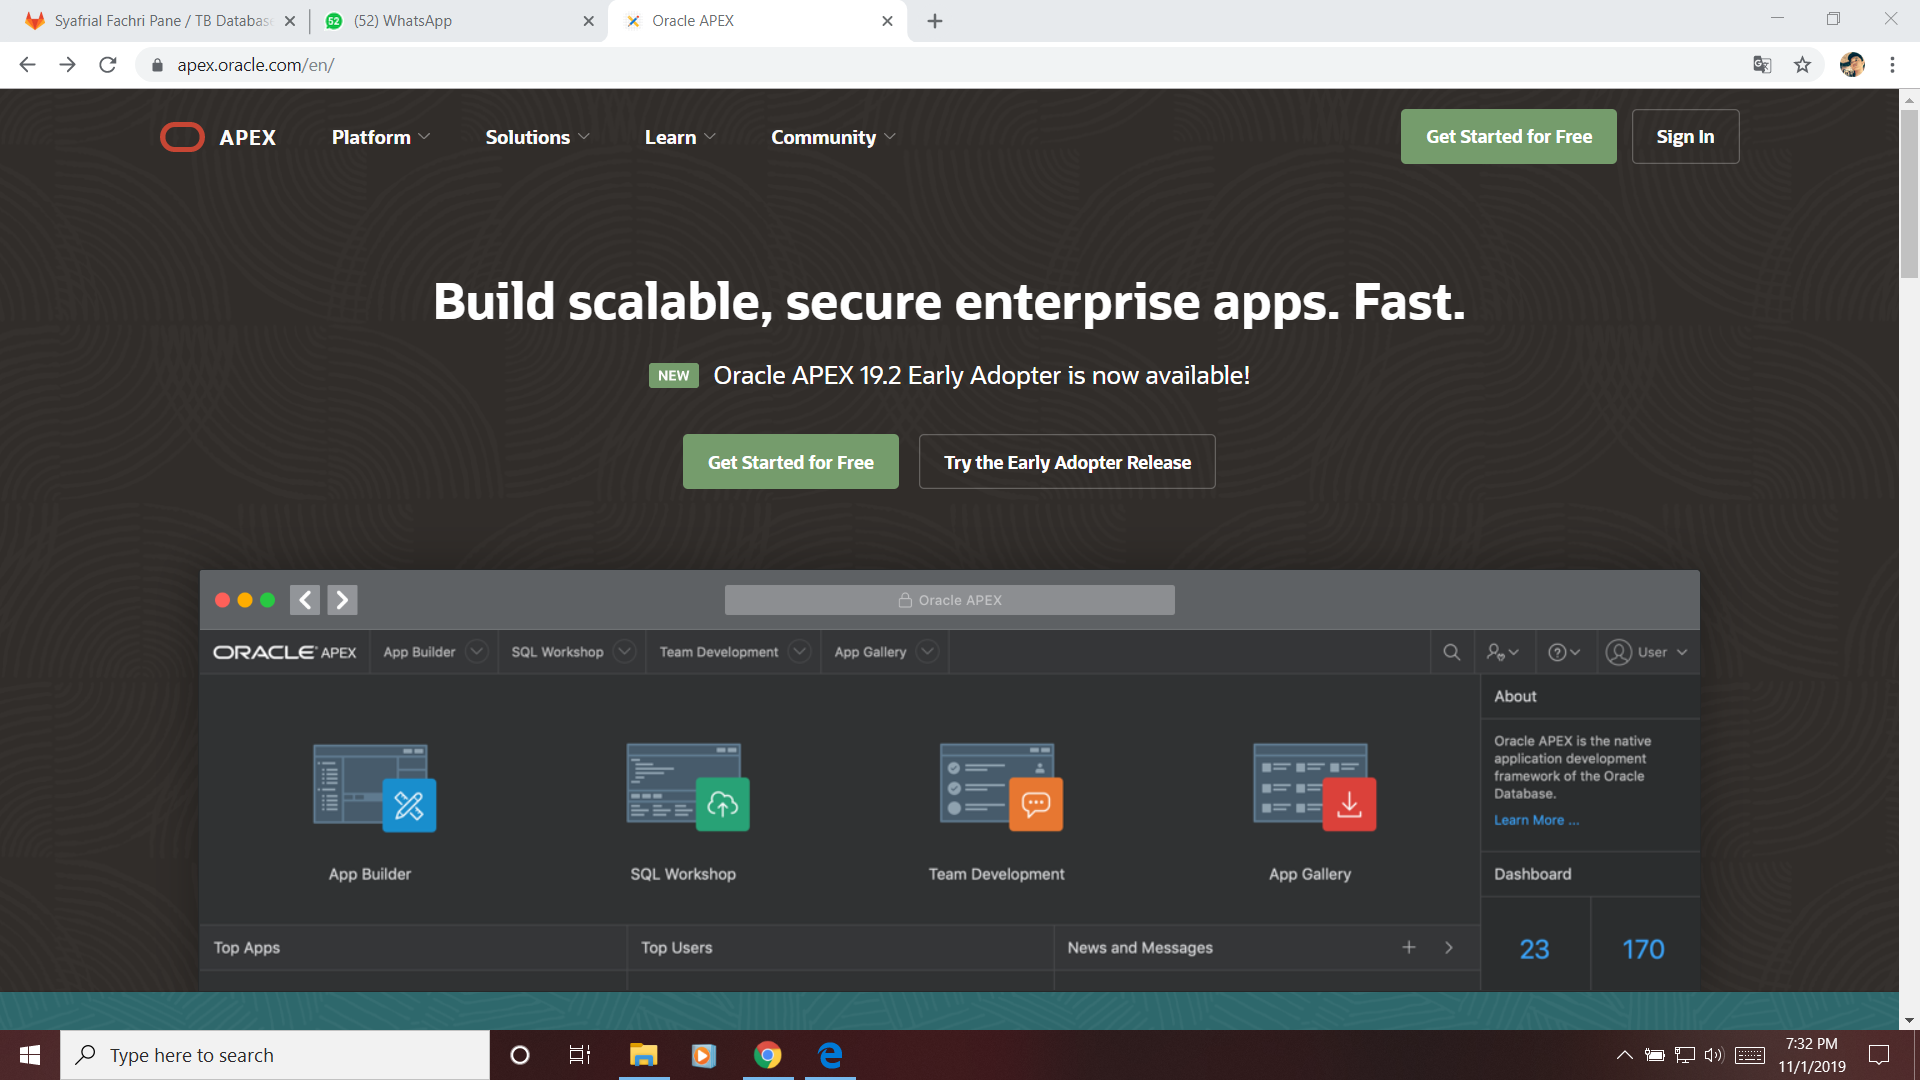
\includegraphics[scale=0.2]{Gambar/Capture1}
	\caption{•}
\end{figure}
\item LOGIN menggunakan workspace yang sudah kalian gunakan
\begin{figure}[h]
	\centering
		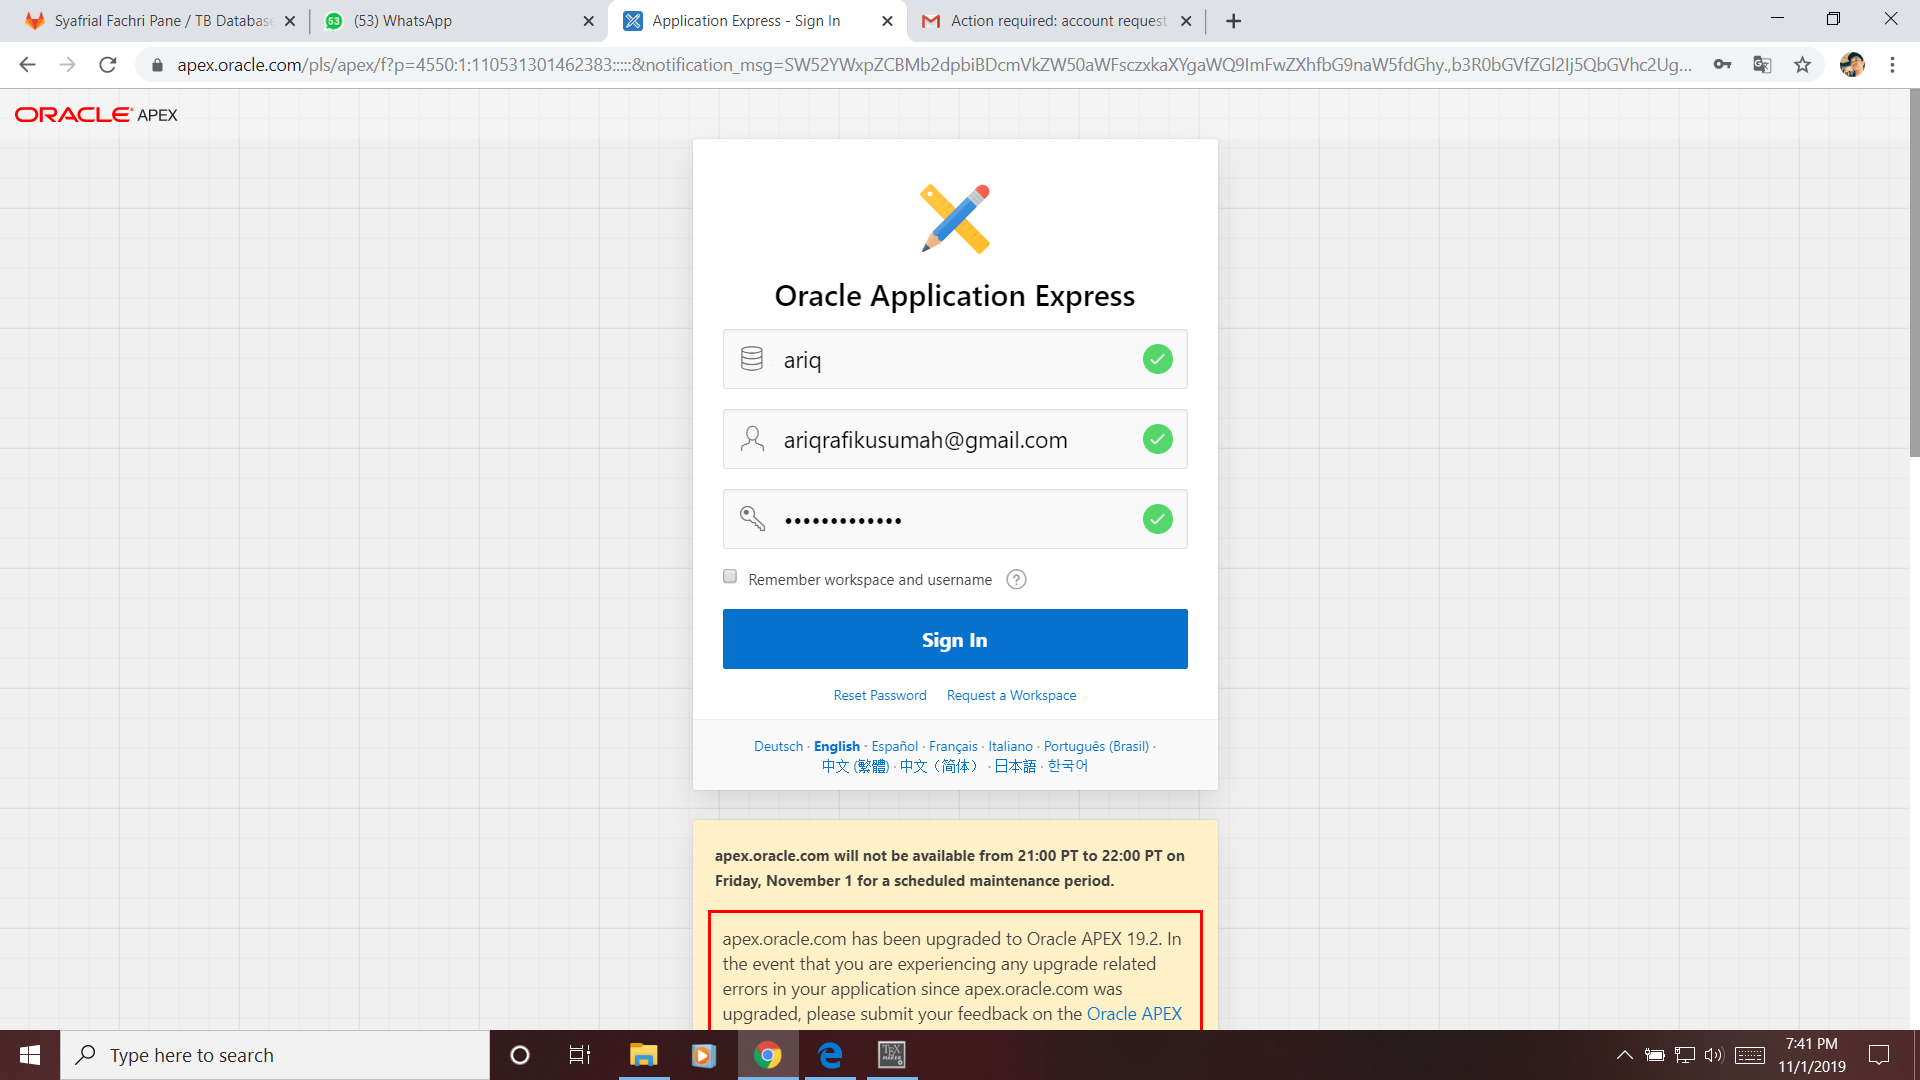
\includegraphics[scale=0.2]{Gambar/Capture2}
	\caption{•}
\end{figure}
\\
\\
\item Pilih App Builder
\begin{figure}[h]
	\centering
		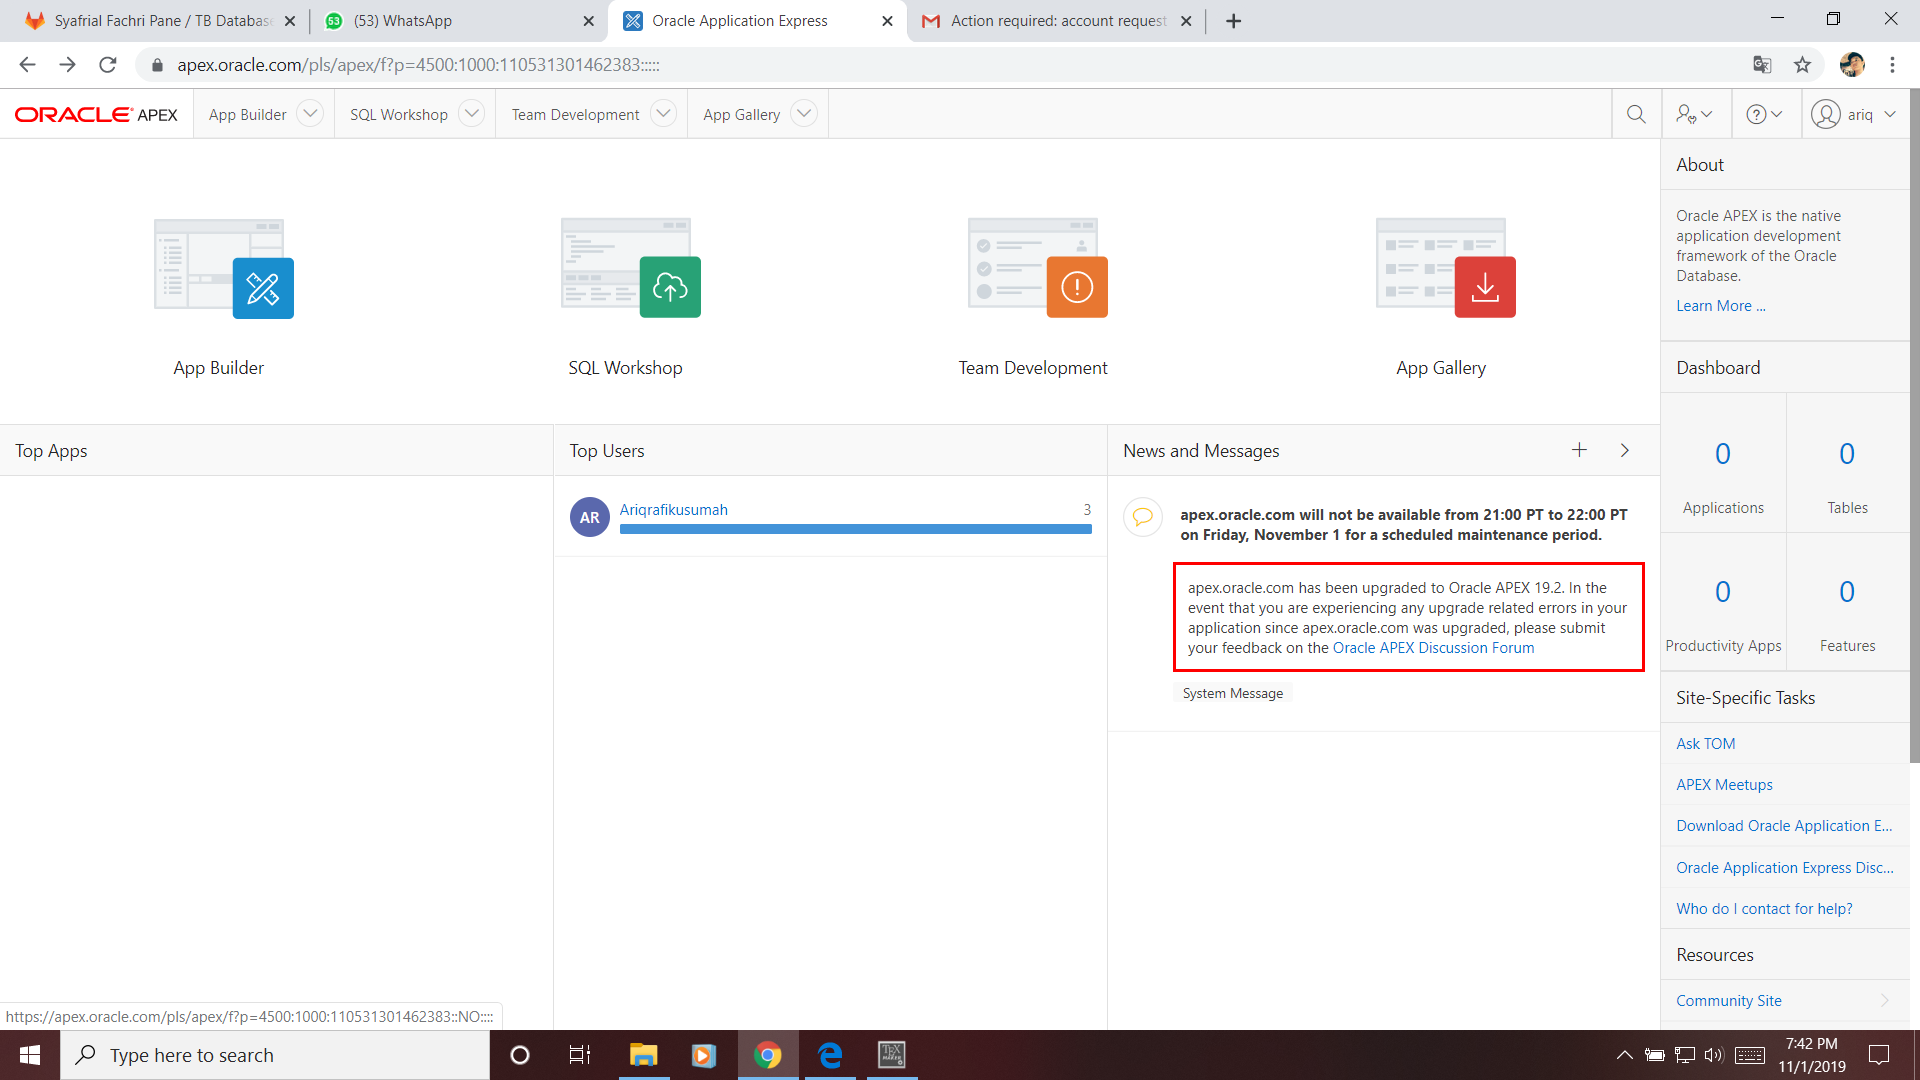
\includegraphics[scale=0.2]{Gambar/Capture3}
	\caption{•}
\end{figure}
\item Pilih create 
\begin{figure}[h]
	\centering
		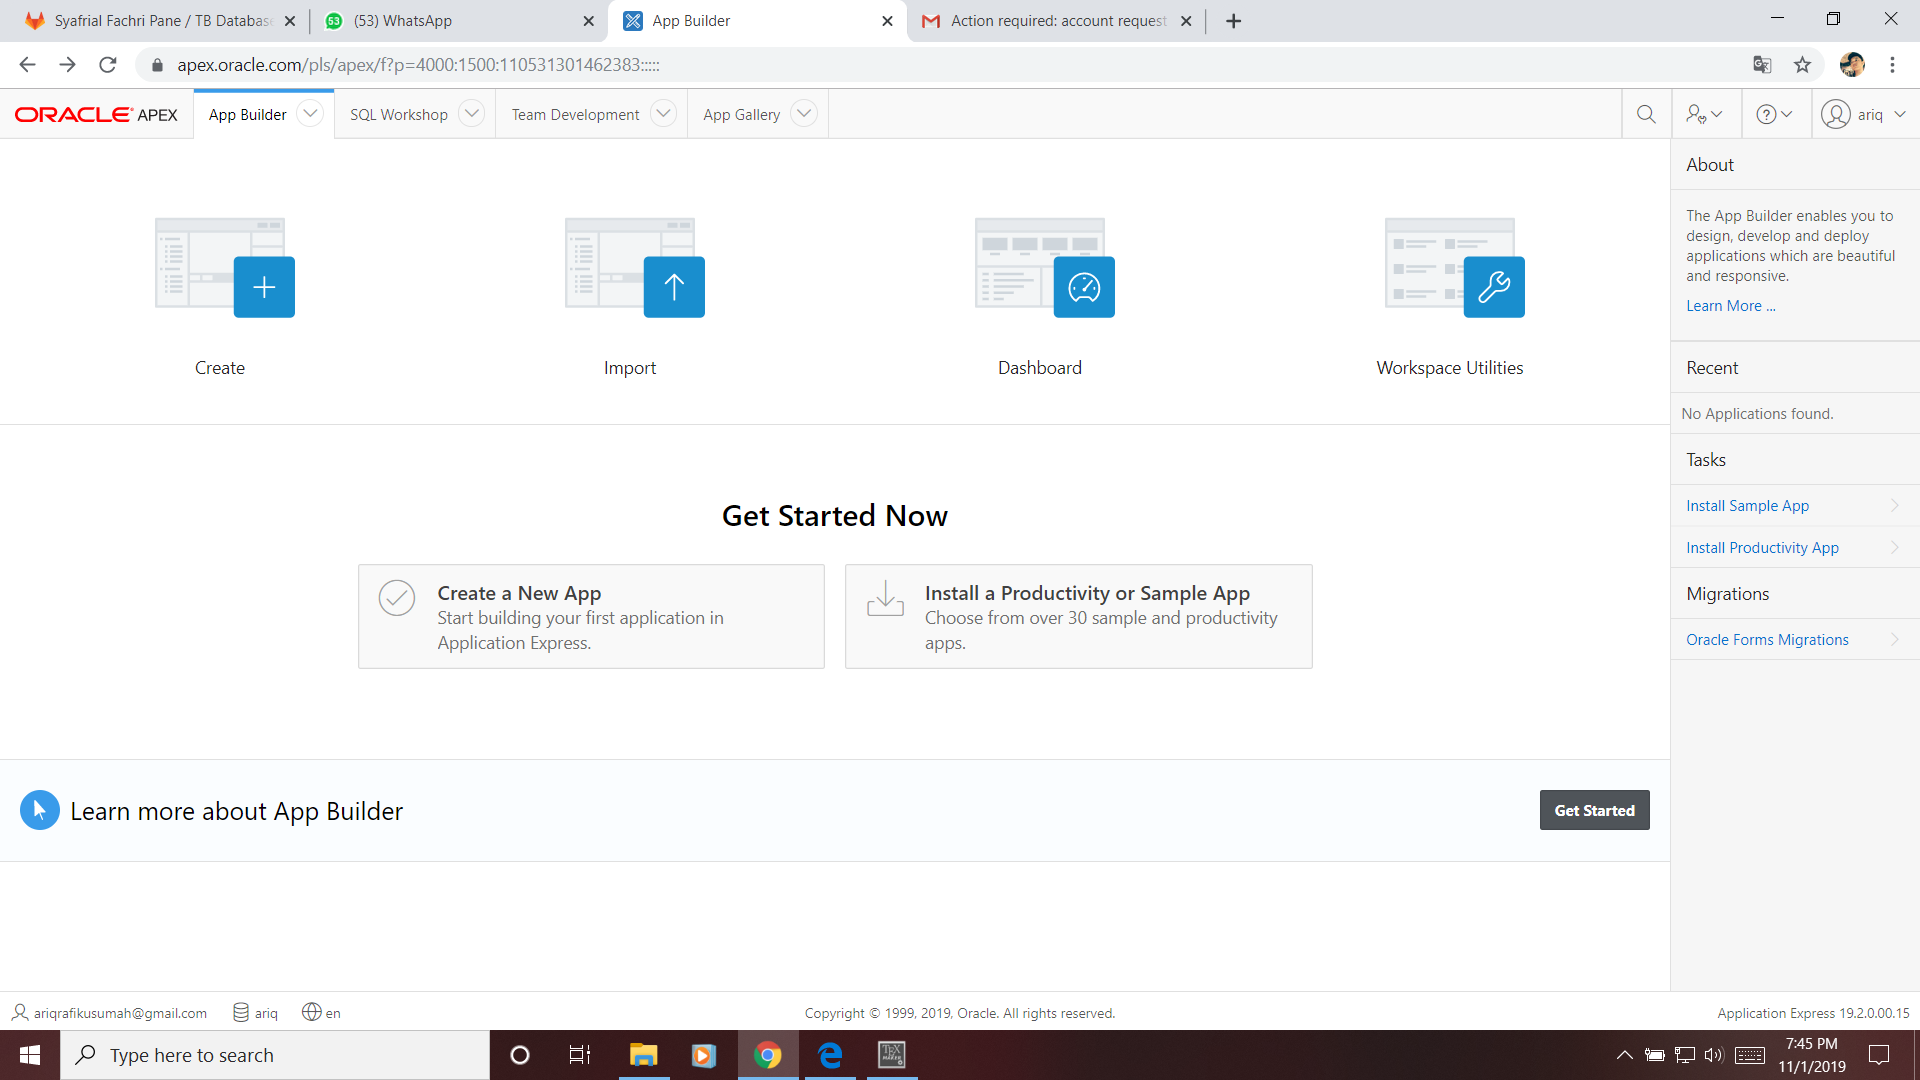
\includegraphics[scale=0.2]{Gambar/Capture4}
	\caption{•}
\end{figure}
\\
\\
\\
\\
\\
\\
\\
\\
\\
\\
\\
\item Pilih Import File
\begin{figure}[h]
	\centering
		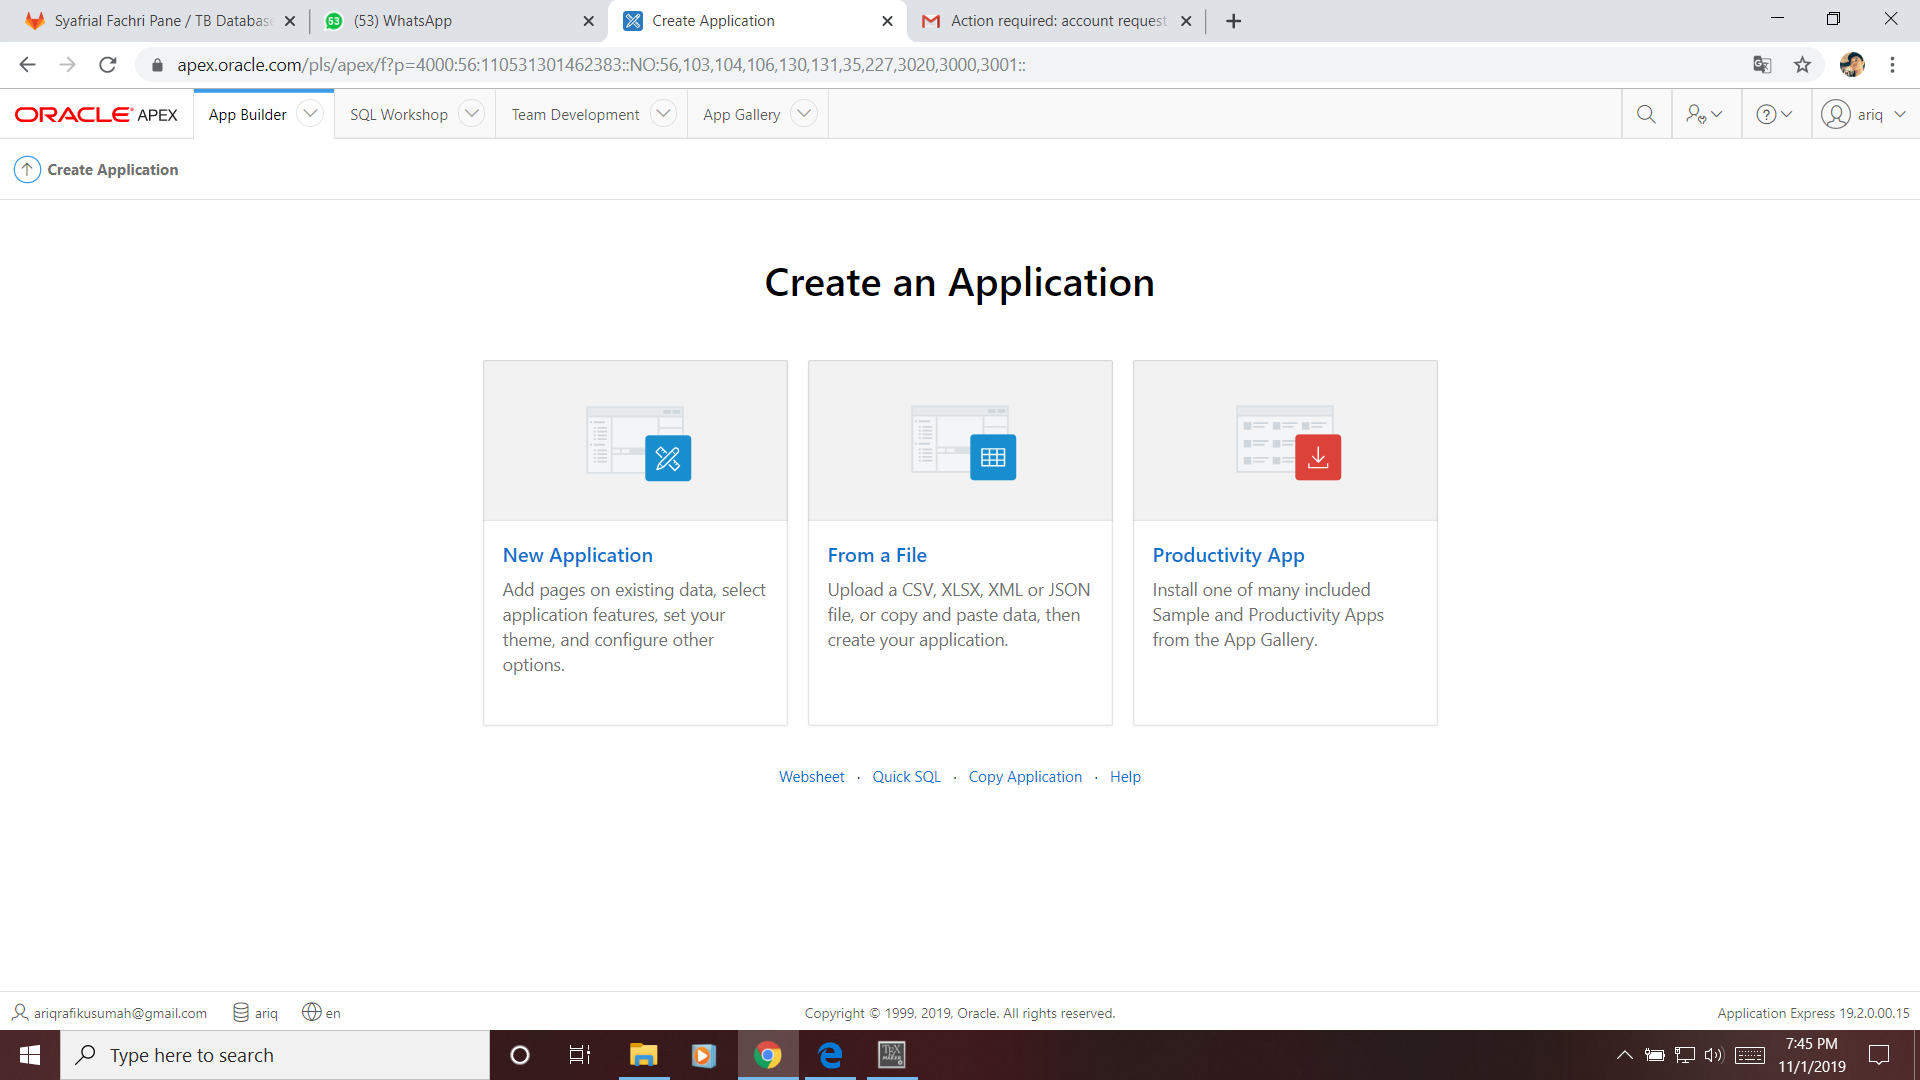
\includegraphics[scale=0.2]{Gambar/Capture5}
	\caption{•}
\end{figure}
\item Drag and drop file yang telah dibuat
\begin{figure}[h]
	\centering
		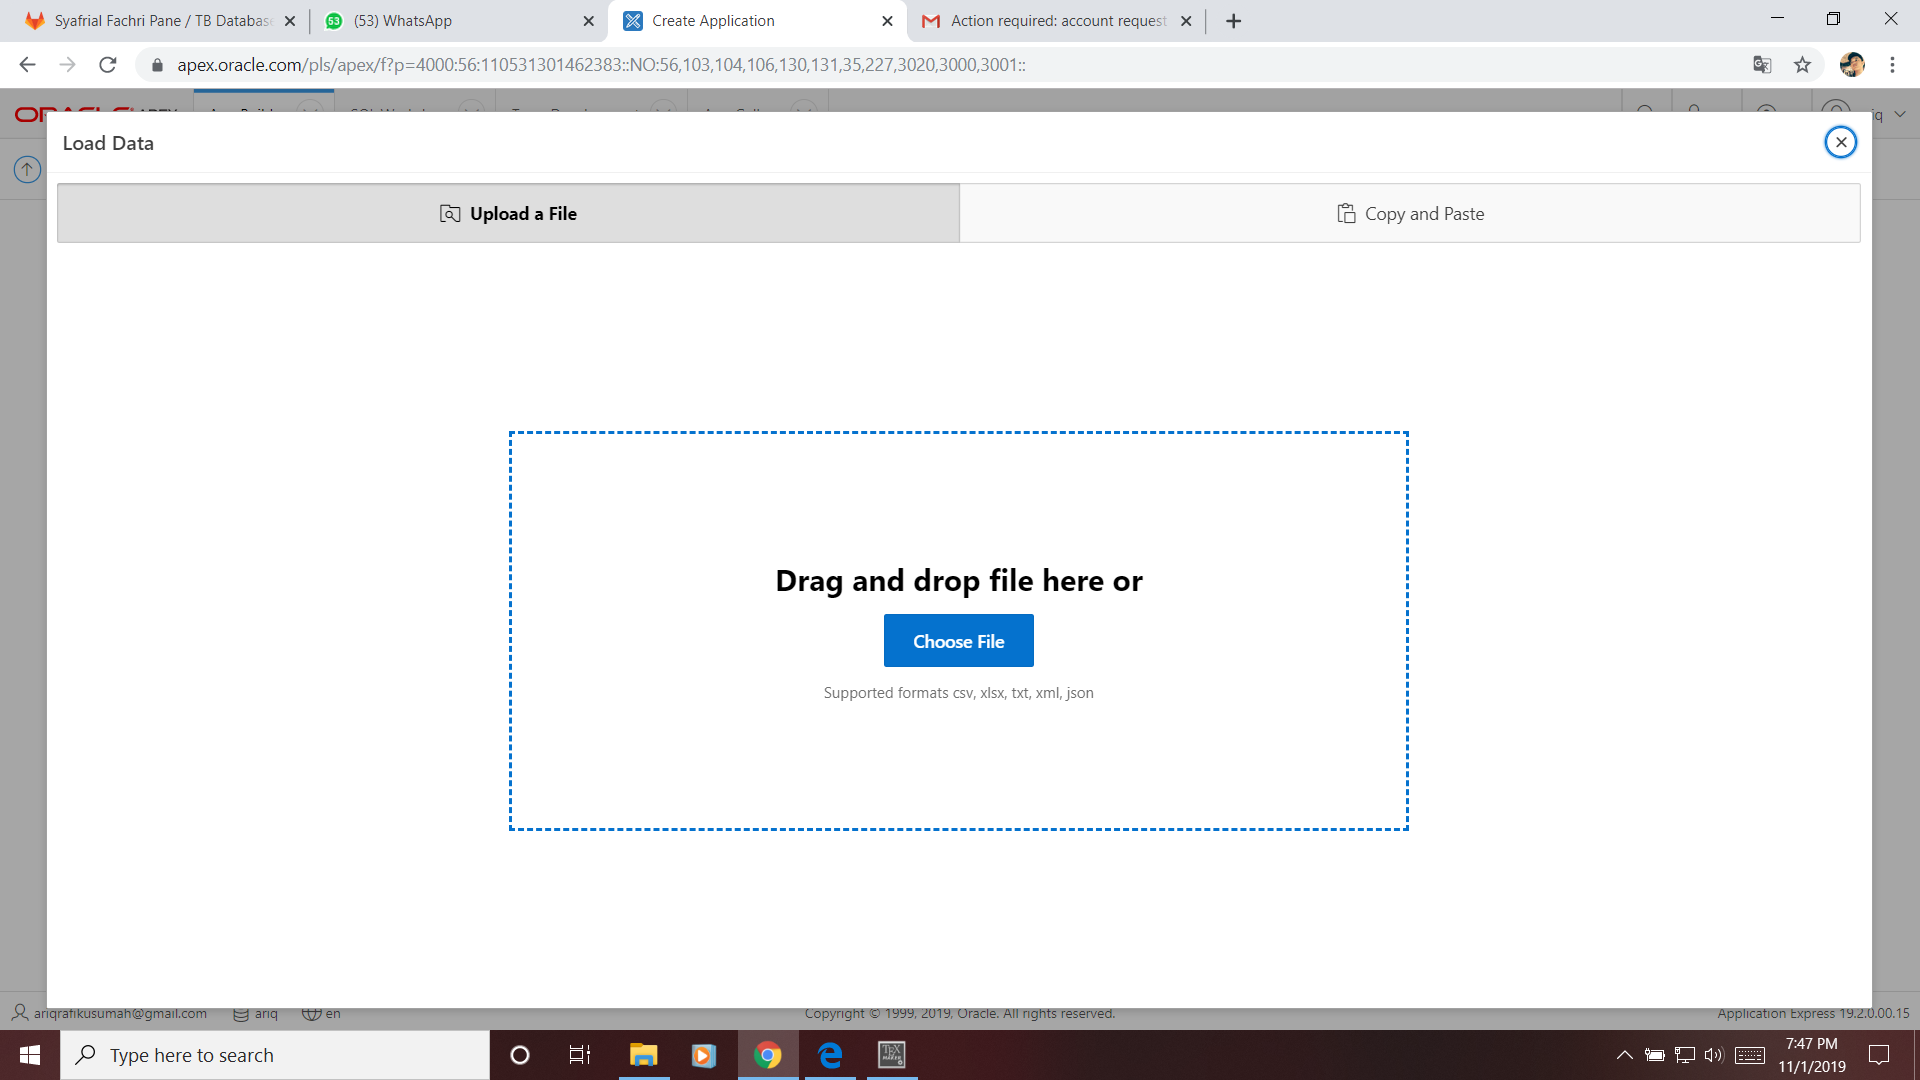
\includegraphics[scale=0.2]{Gambar/Capture6}
	\caption{•}
\end{figure}
\\
\\
\\
\\
\\
\\
\\
\\
\\
\\
\\
\\
\\
\item Buat Nama tabel nya
\begin{figure}[h]
	\centering
		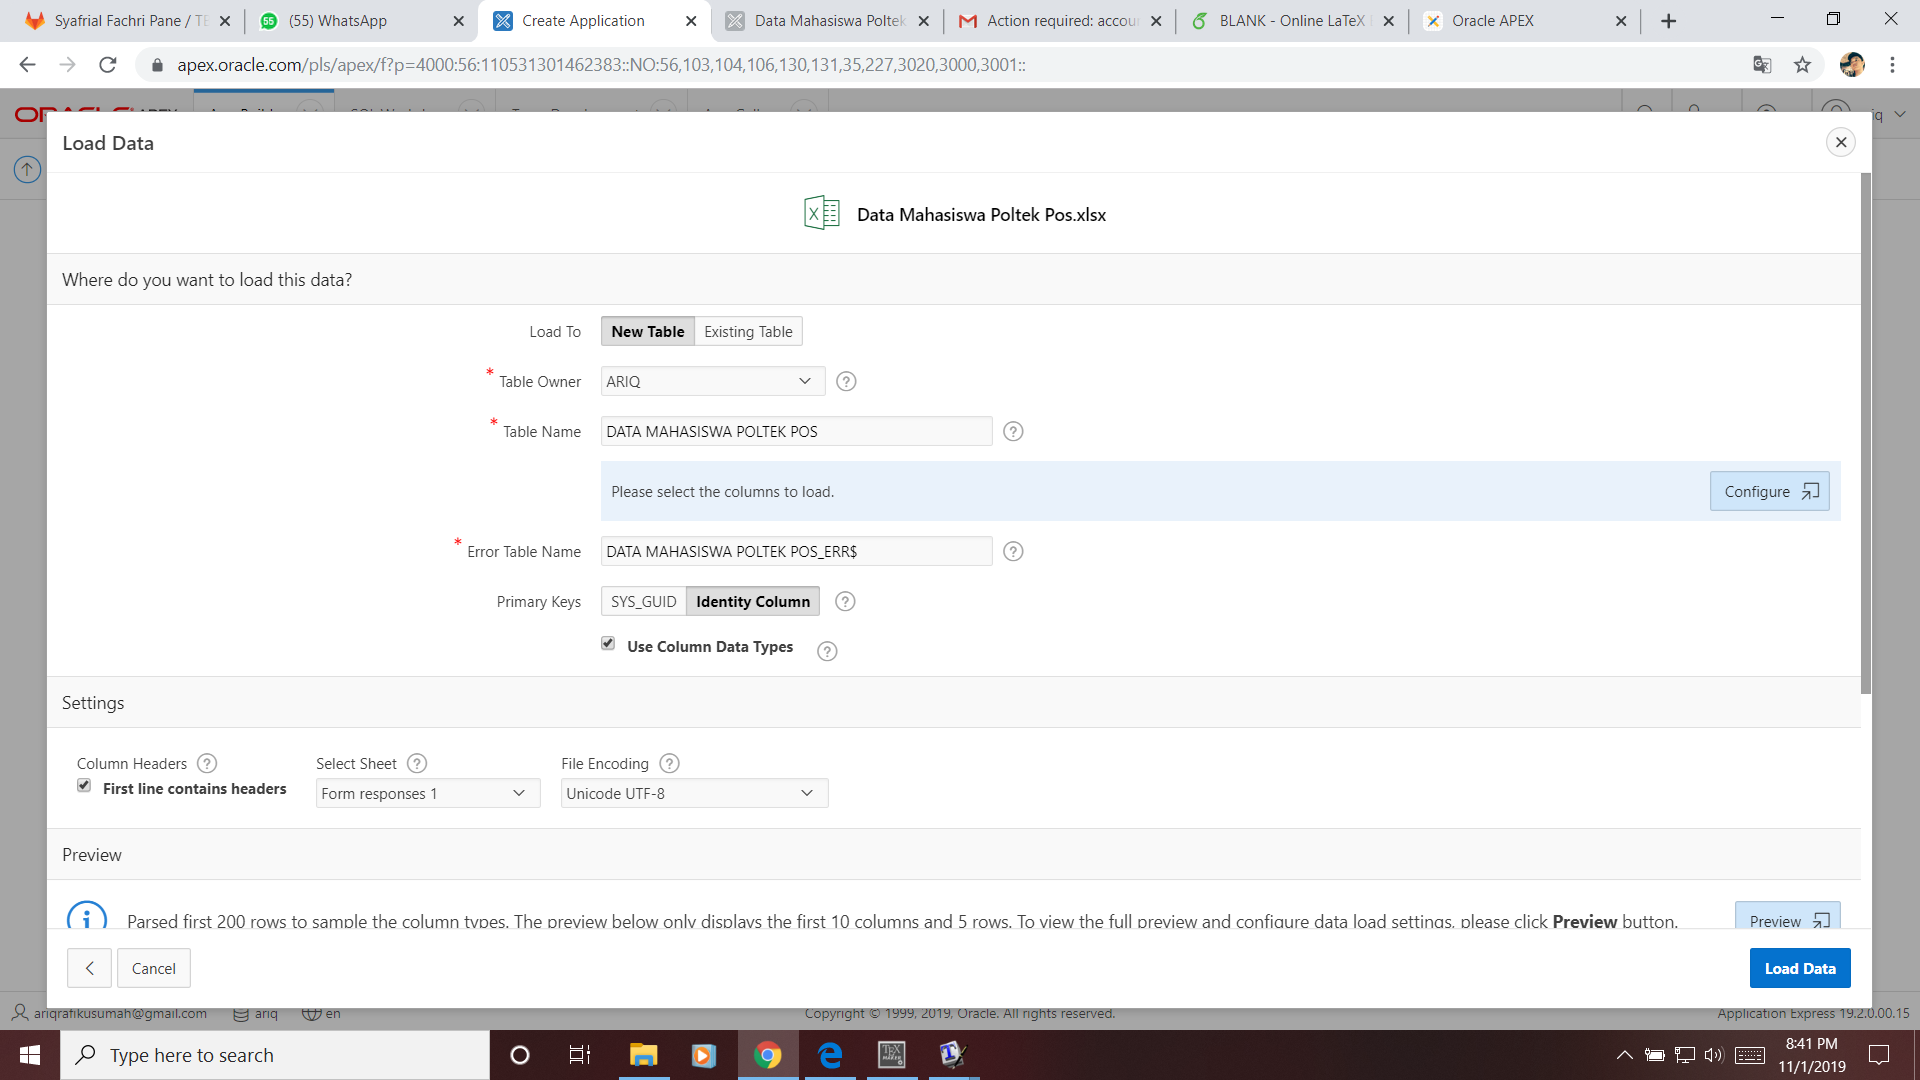
\includegraphics[scale=0.2]{Gambar/Capture7}
	\caption{•}
\end{figure}
\item  Setelah itu Scroll kebawah,lalu pilih preview
\begin{figure}[h]
	\centering
		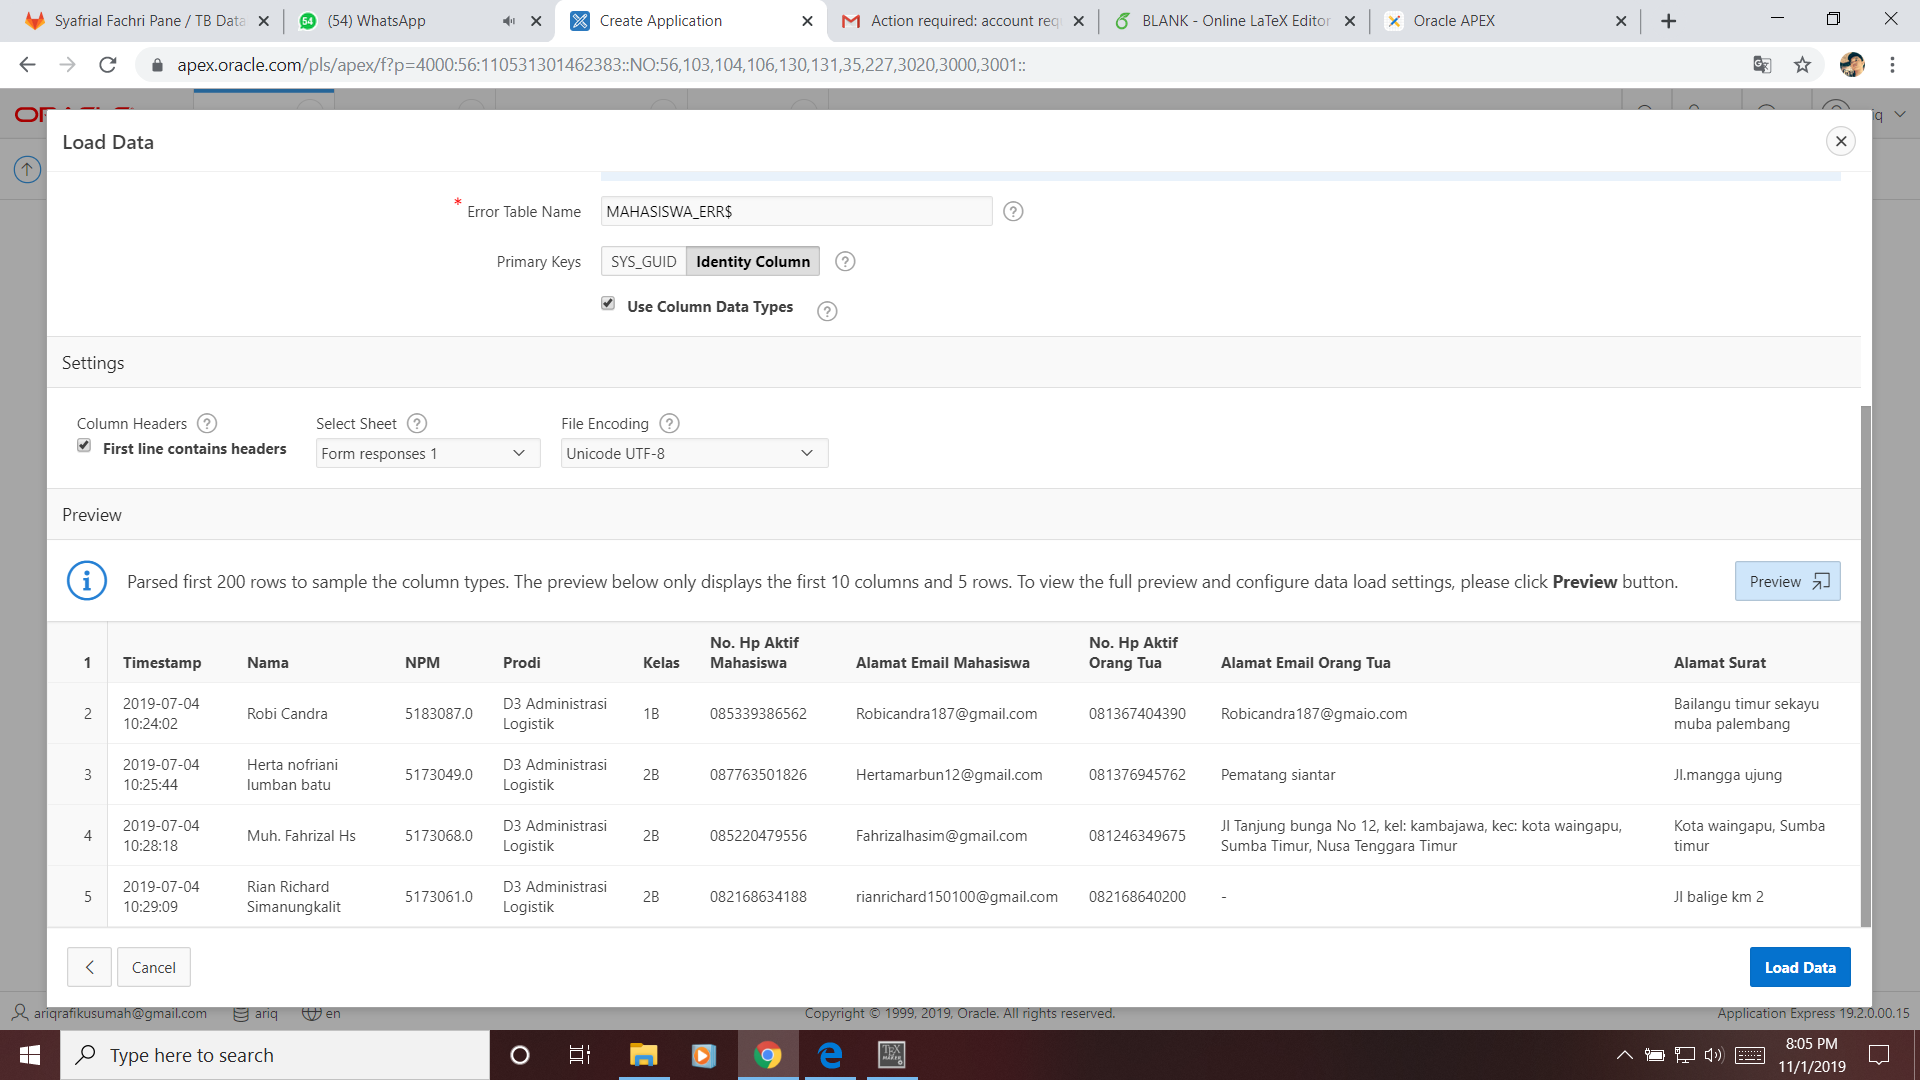
\includegraphics[scale=0.2]{Gambar/Capture8}
	\caption{•}
\end{figure}
\\
\\
\\
\\
\\
\\
\\
\\
\\
\\
\\
\\
\\
\item  Melihat data yang telah kalian masukkan
\begin{figure}[h]
	\centering
		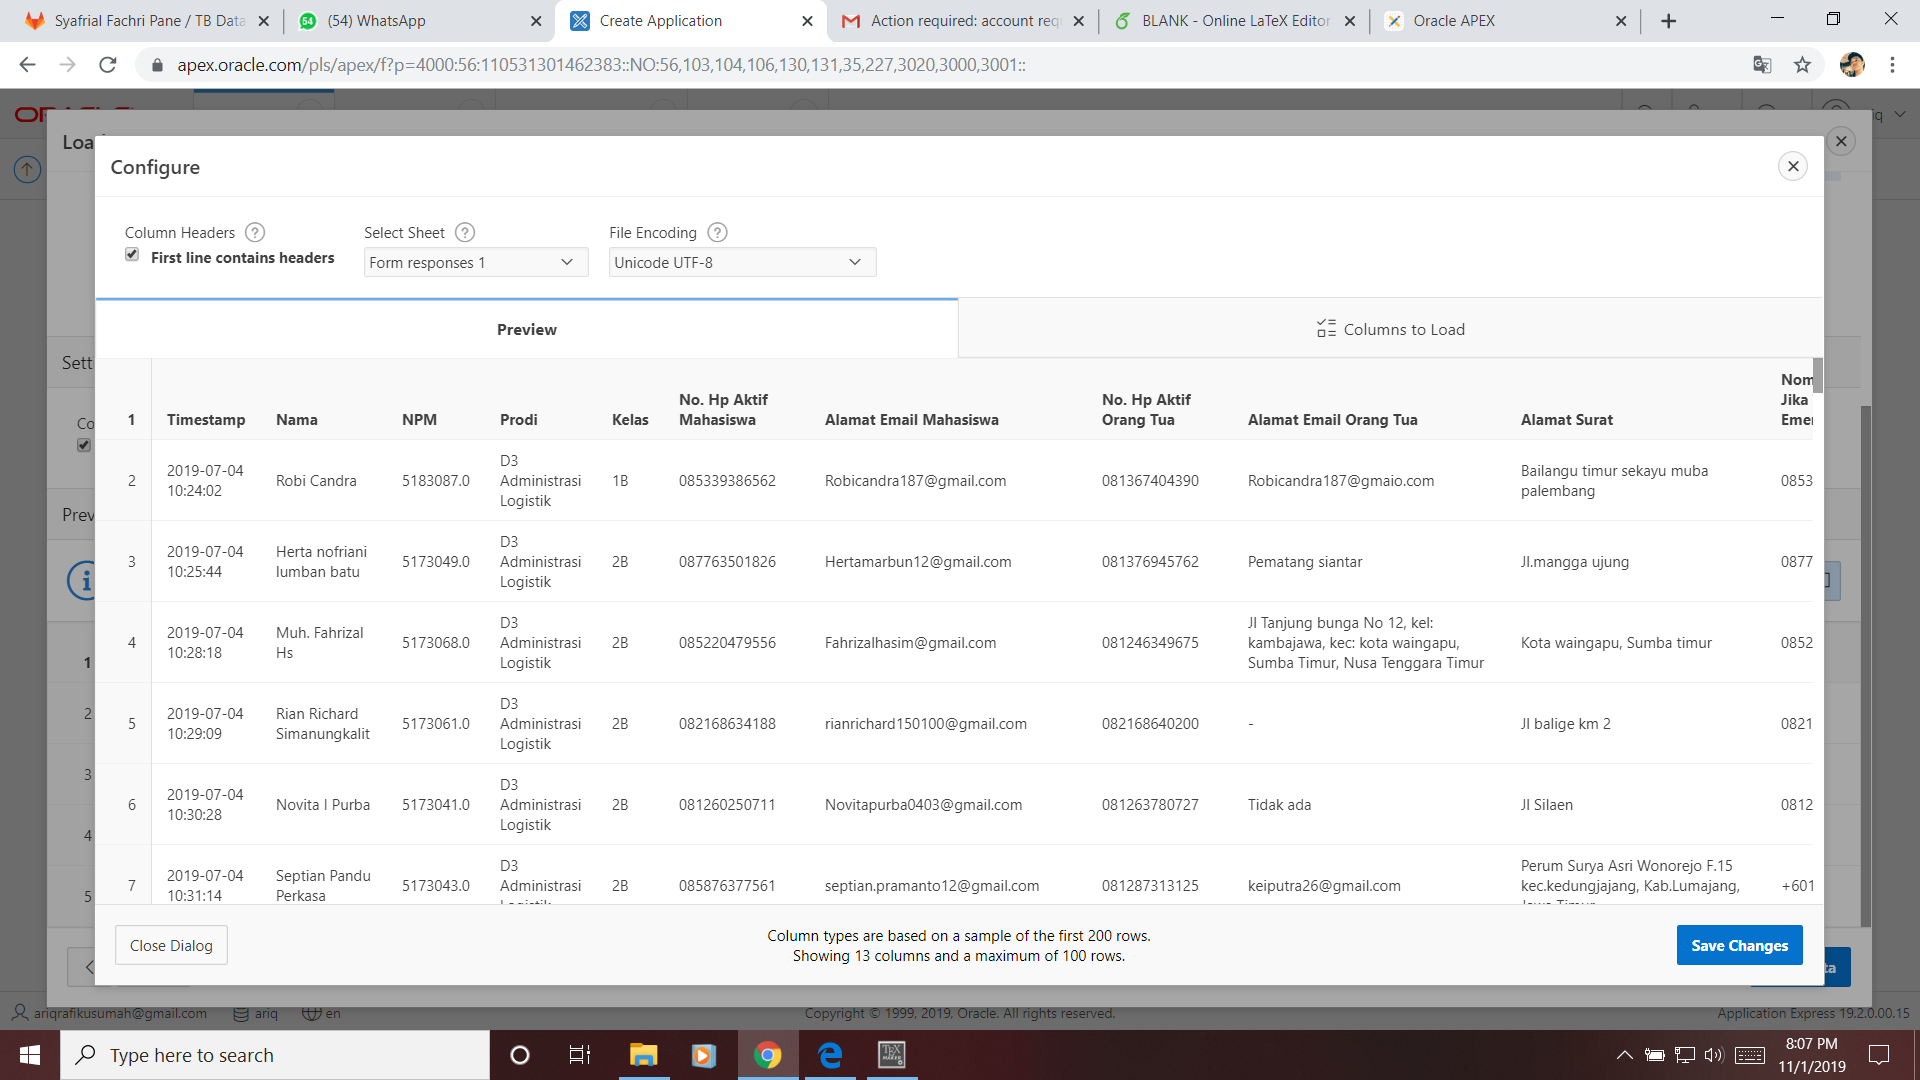
\includegraphics[scale=0.2]{Gambar/Capture9}
	\caption{•}
\end{figure}
\item lalu pilih column to load untuk melihat nama column dan pilih save change
\begin{figure}[h]
	\centering
		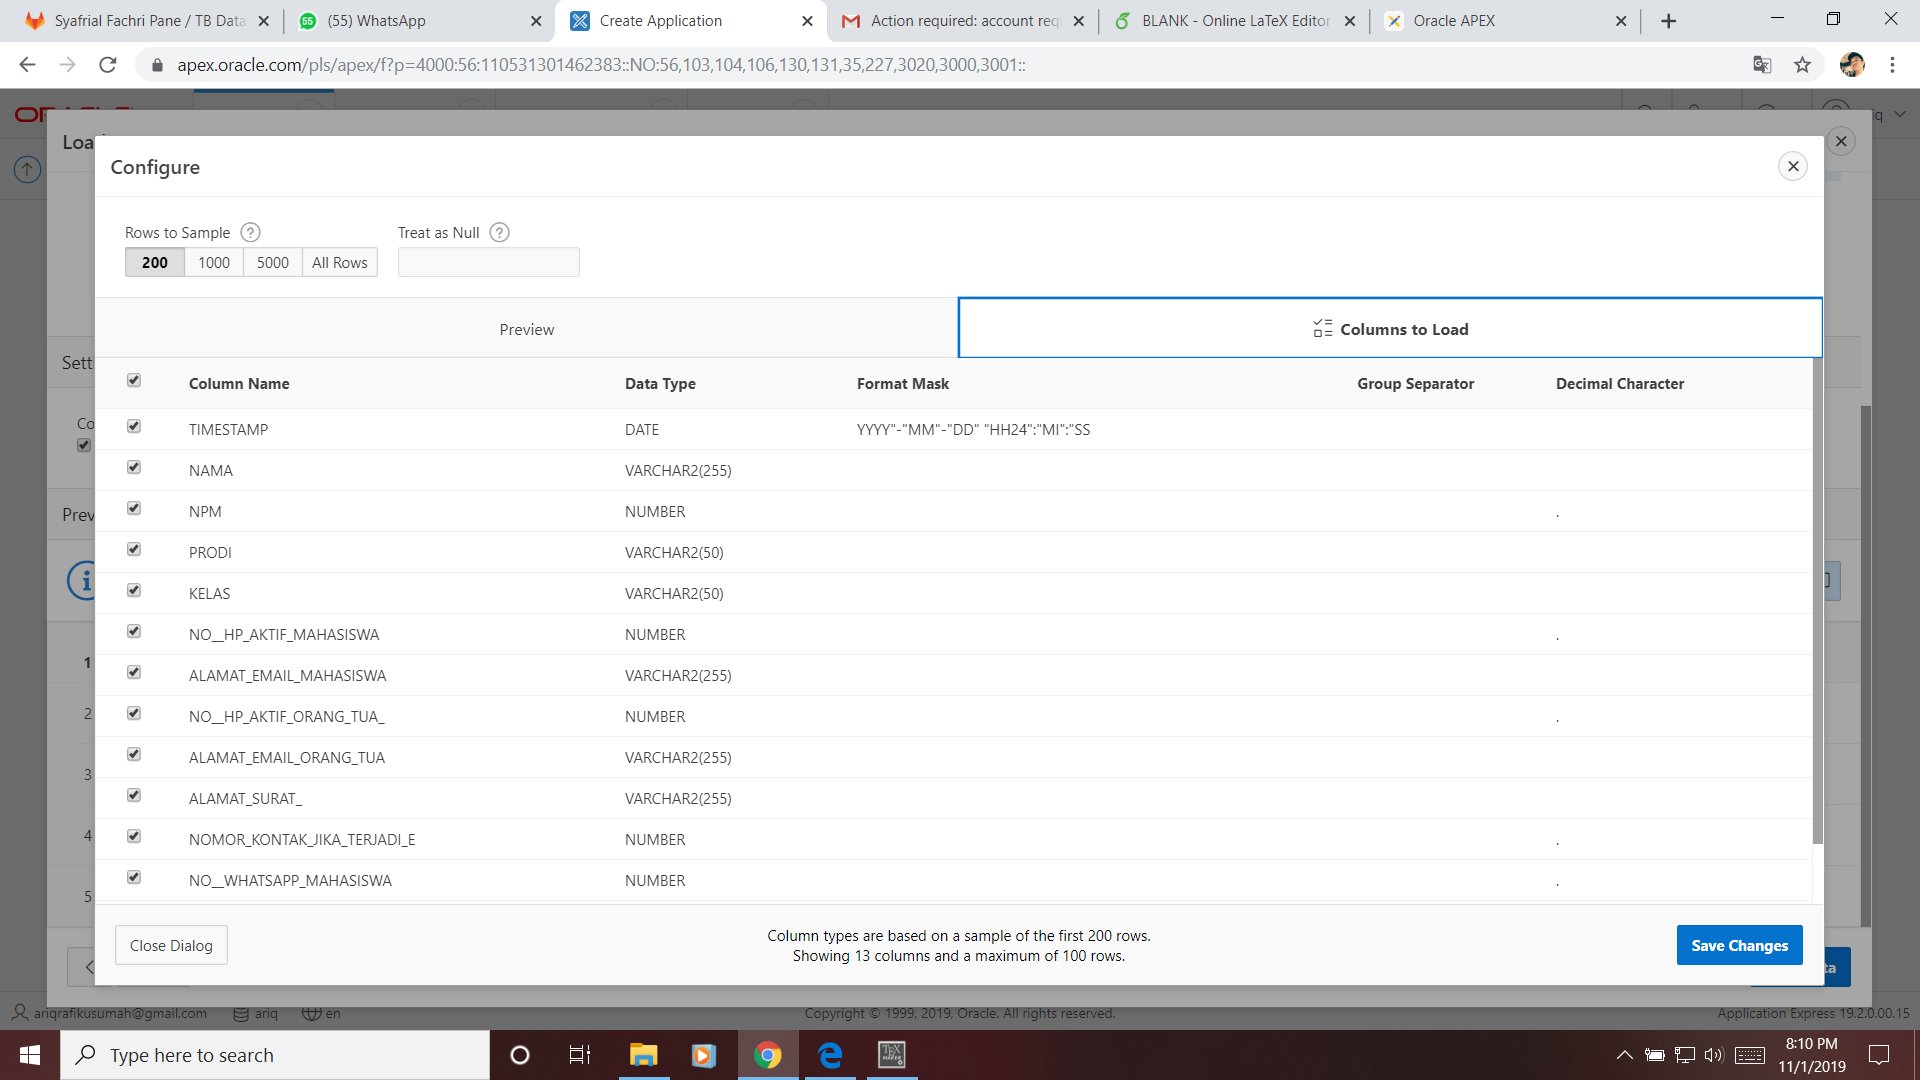
\includegraphics[scale=0.2]{Gambar/Capture10}
	\caption{•}
\end{figure}
\\
\\
\\
\\
\\
\\
\\
\\
\\
\\
\\
\\
\item Pilih Create application
\begin{figure}[h]
	\centering
		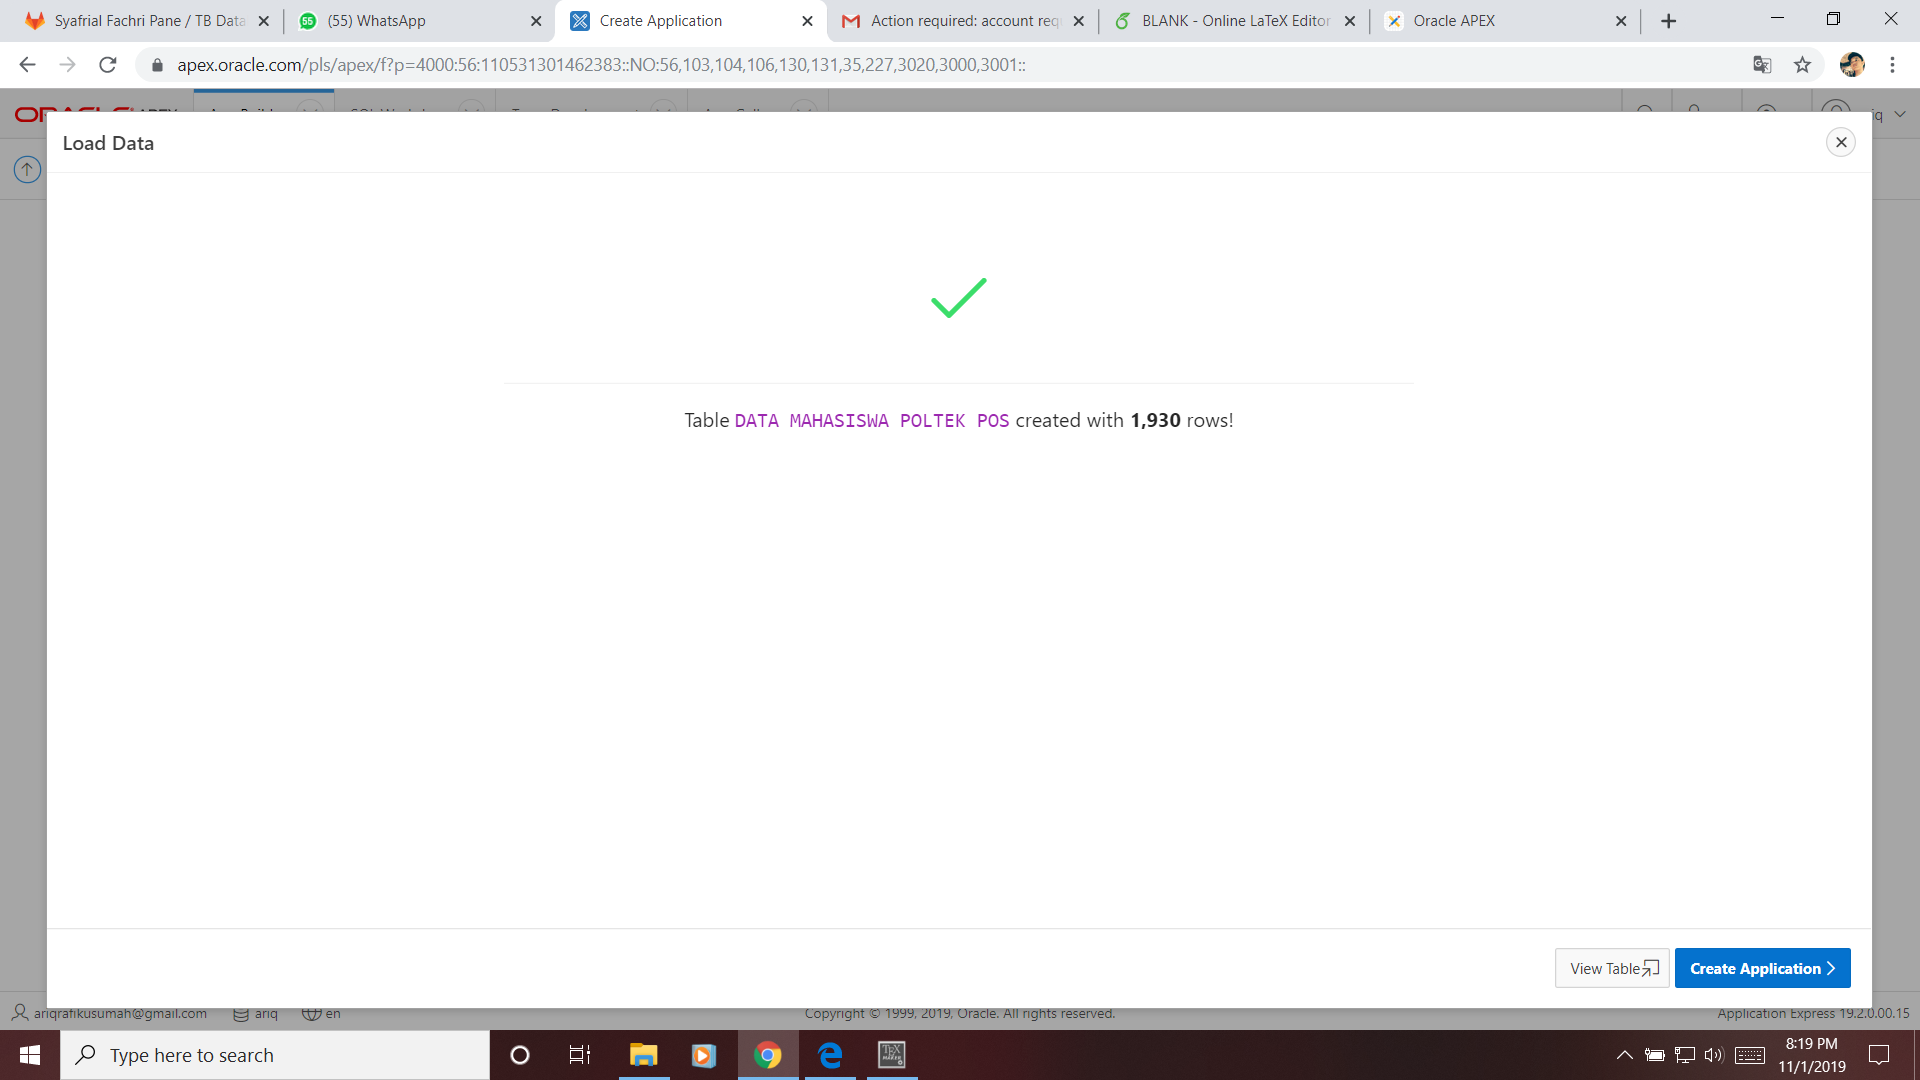
\includegraphics[scale=0.2]{Gambar/Capture11}
	\caption{•}
\end{figure}
\item Ceklis semua pada gambar berikut
\begin{figure}[h]
	\centering
		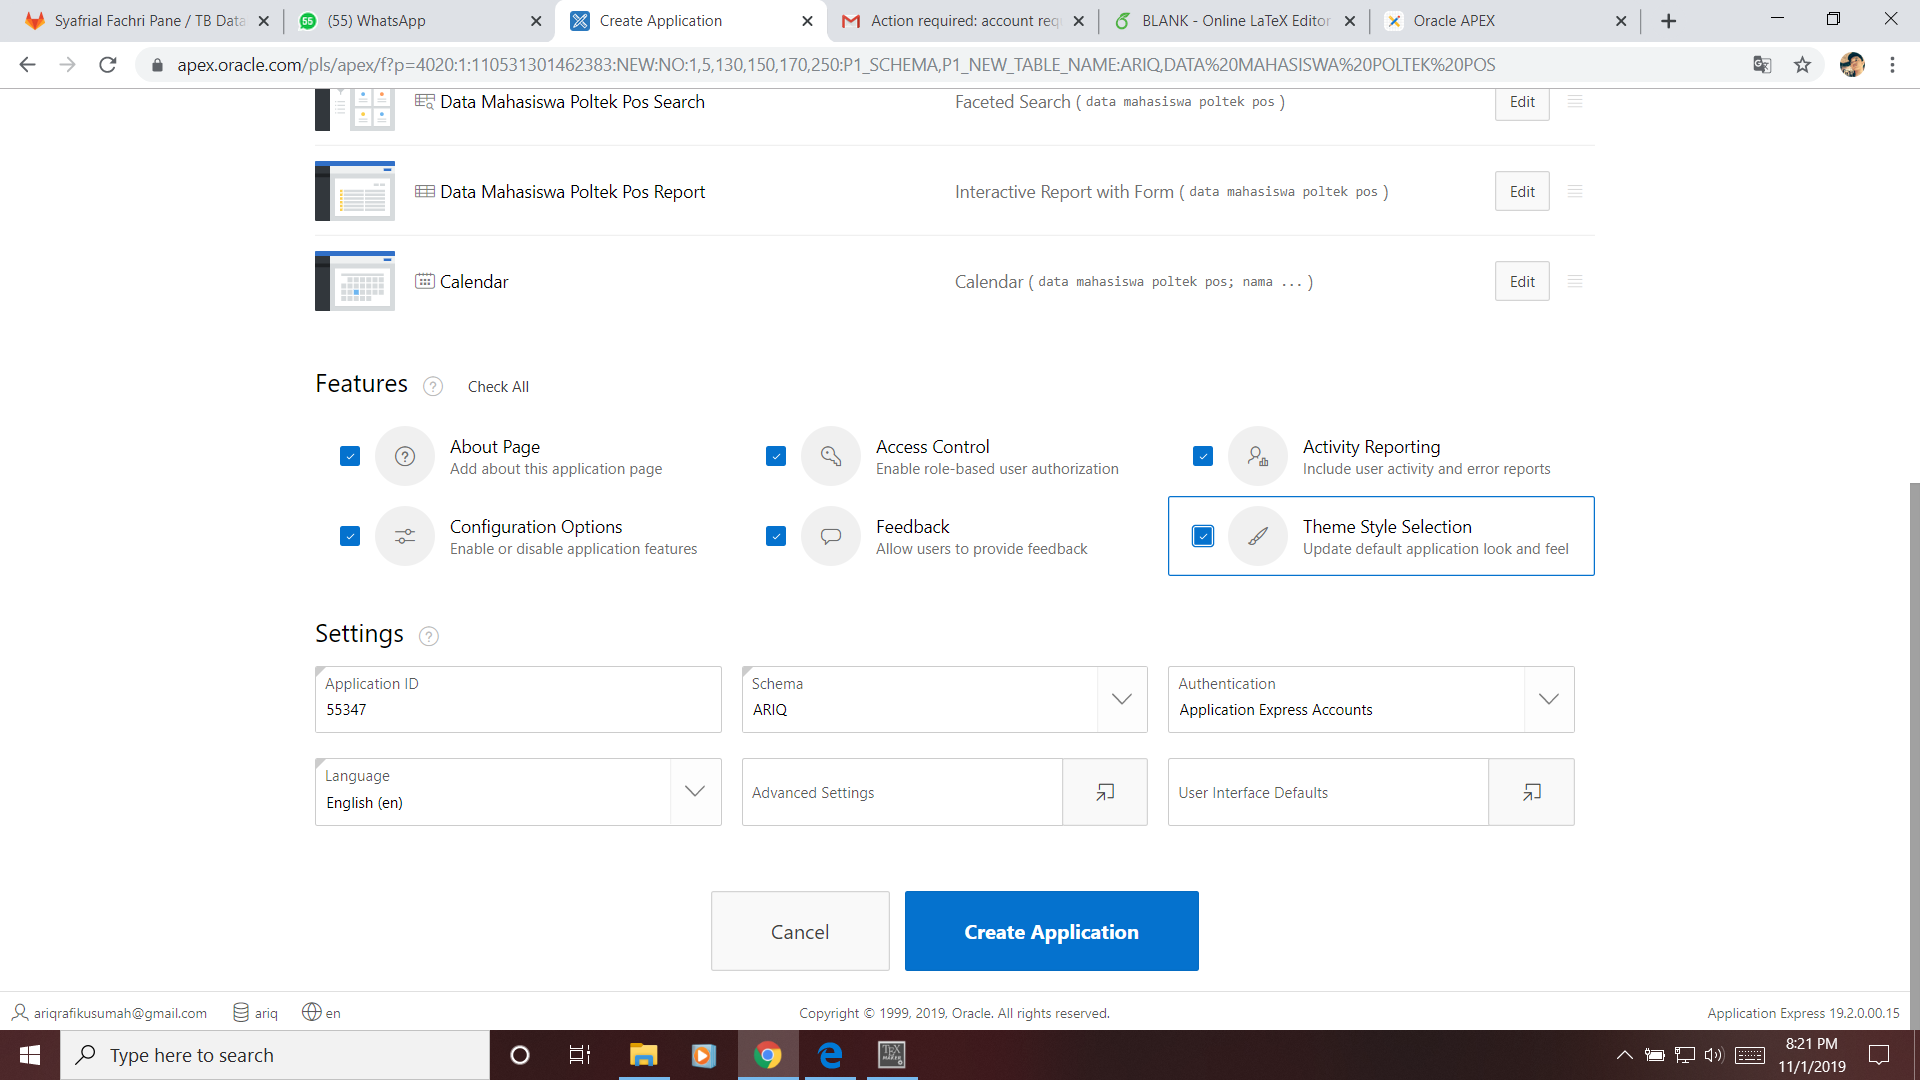
\includegraphics[scale=0.2]{Gambar/Capture12}
	\caption{•}
\end{figure}
\\
\\
\\
\\
\\
\\
\\
\\
\\
\\
\\
\\
\\
\item Tunggu prosses
\begin{figure}[h]
	\centering
		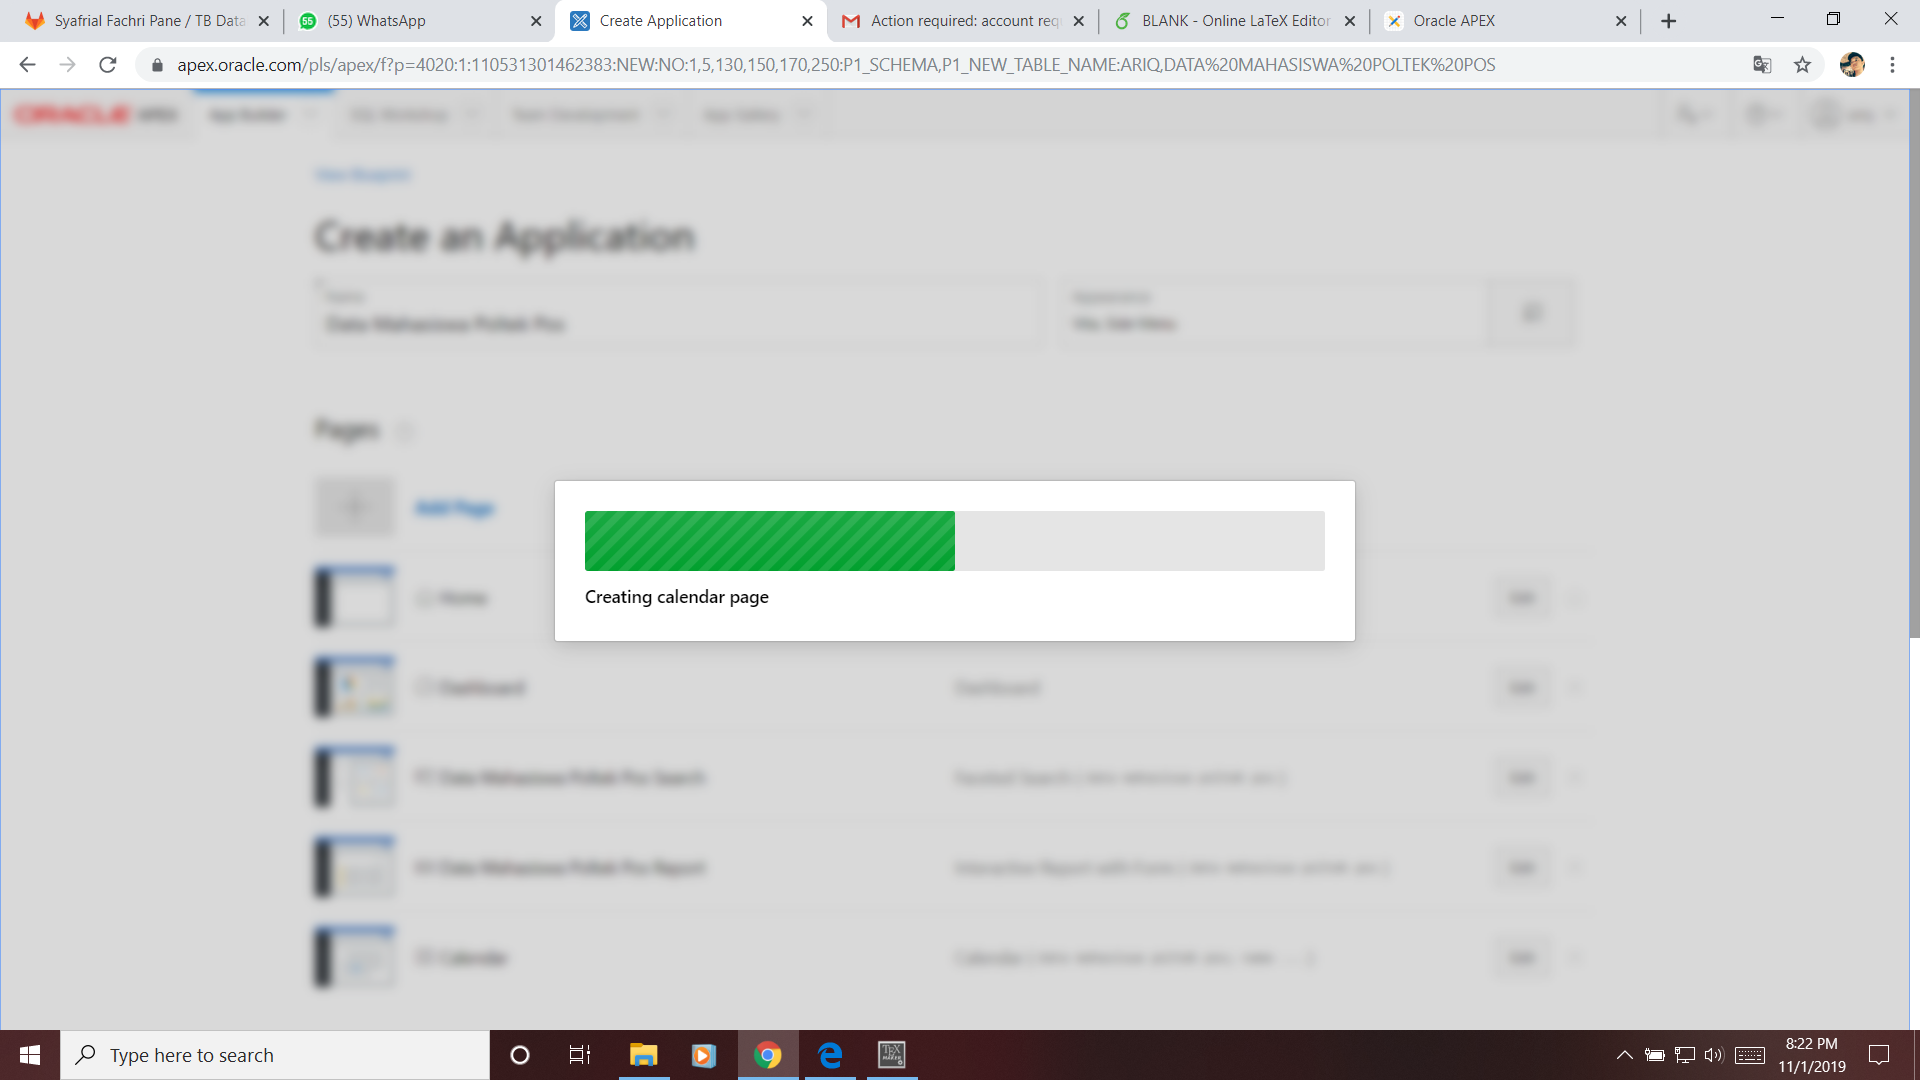
\includegraphics[scale=0.2]{Gambar/Capture13}
	\caption{•}
\end{figure}
\item Pilih Run Application
\begin{figure}[h]
	\centering
		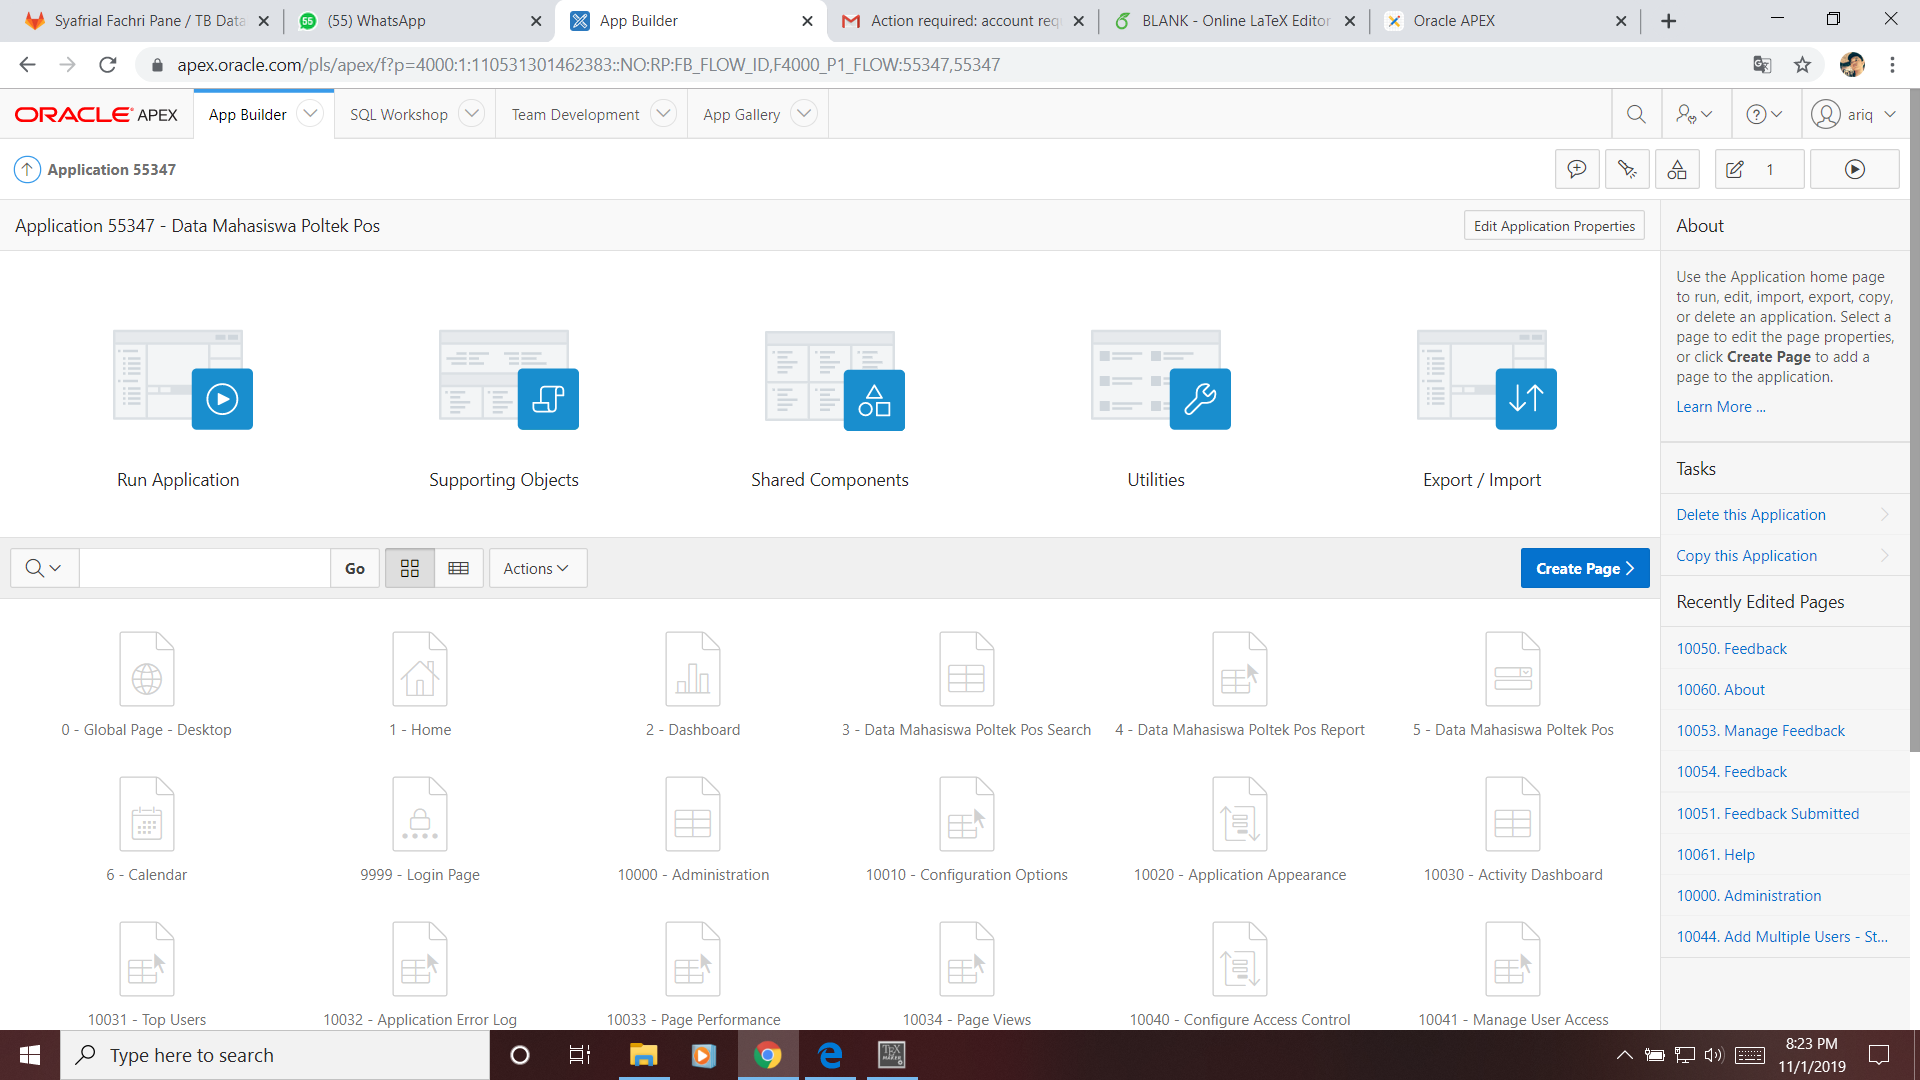
\includegraphics[scale=0.2]{Gambar/Capture14}
	\caption{•}
\end{figure}
\\
\\
\\
\\
\\
\\
\\
\\
\\
\\
\\
\\
\\
\item Login workspace anda buat
\begin{figure}[h]
	\centering
		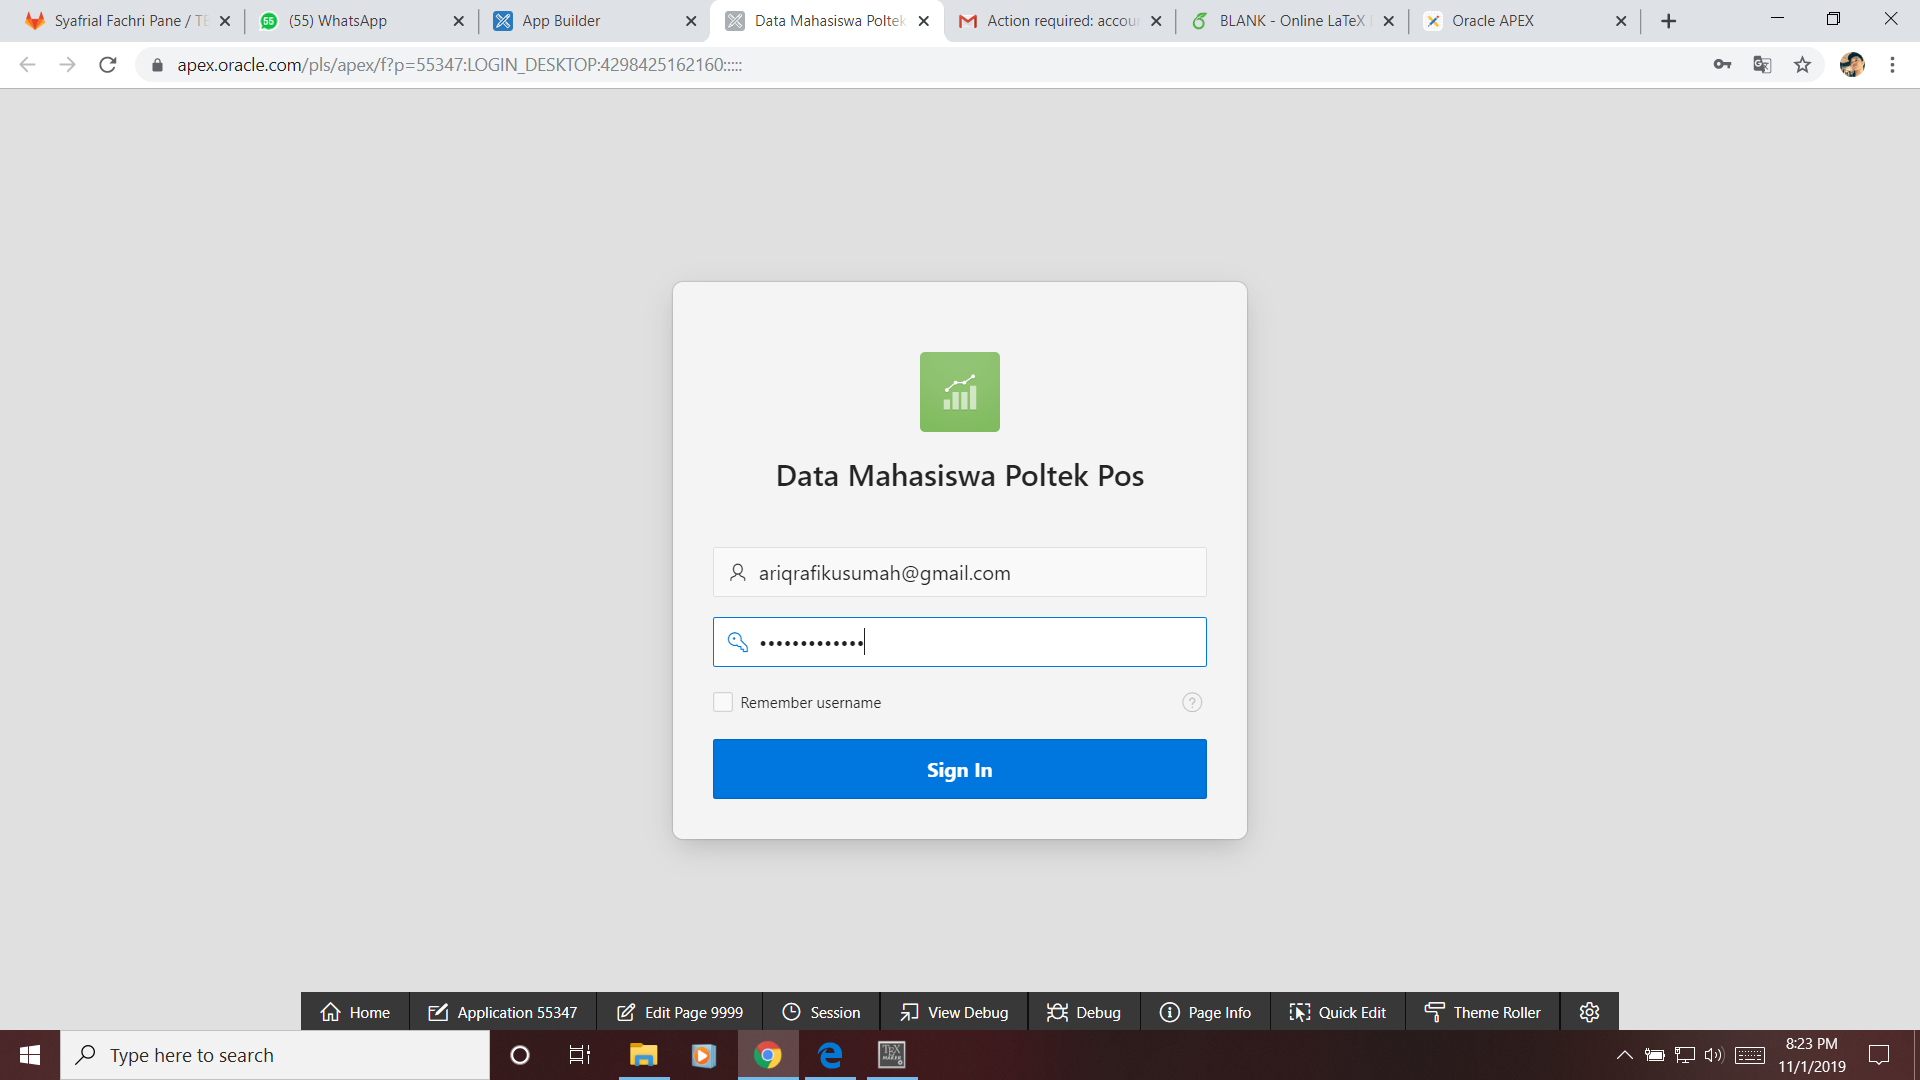
\includegraphics[scale=0.2]{Gambar/Capture15}
	\caption{•}
\end{figure}
\item Berikut tampilan nya
\begin{figure}[h]
	\centering
		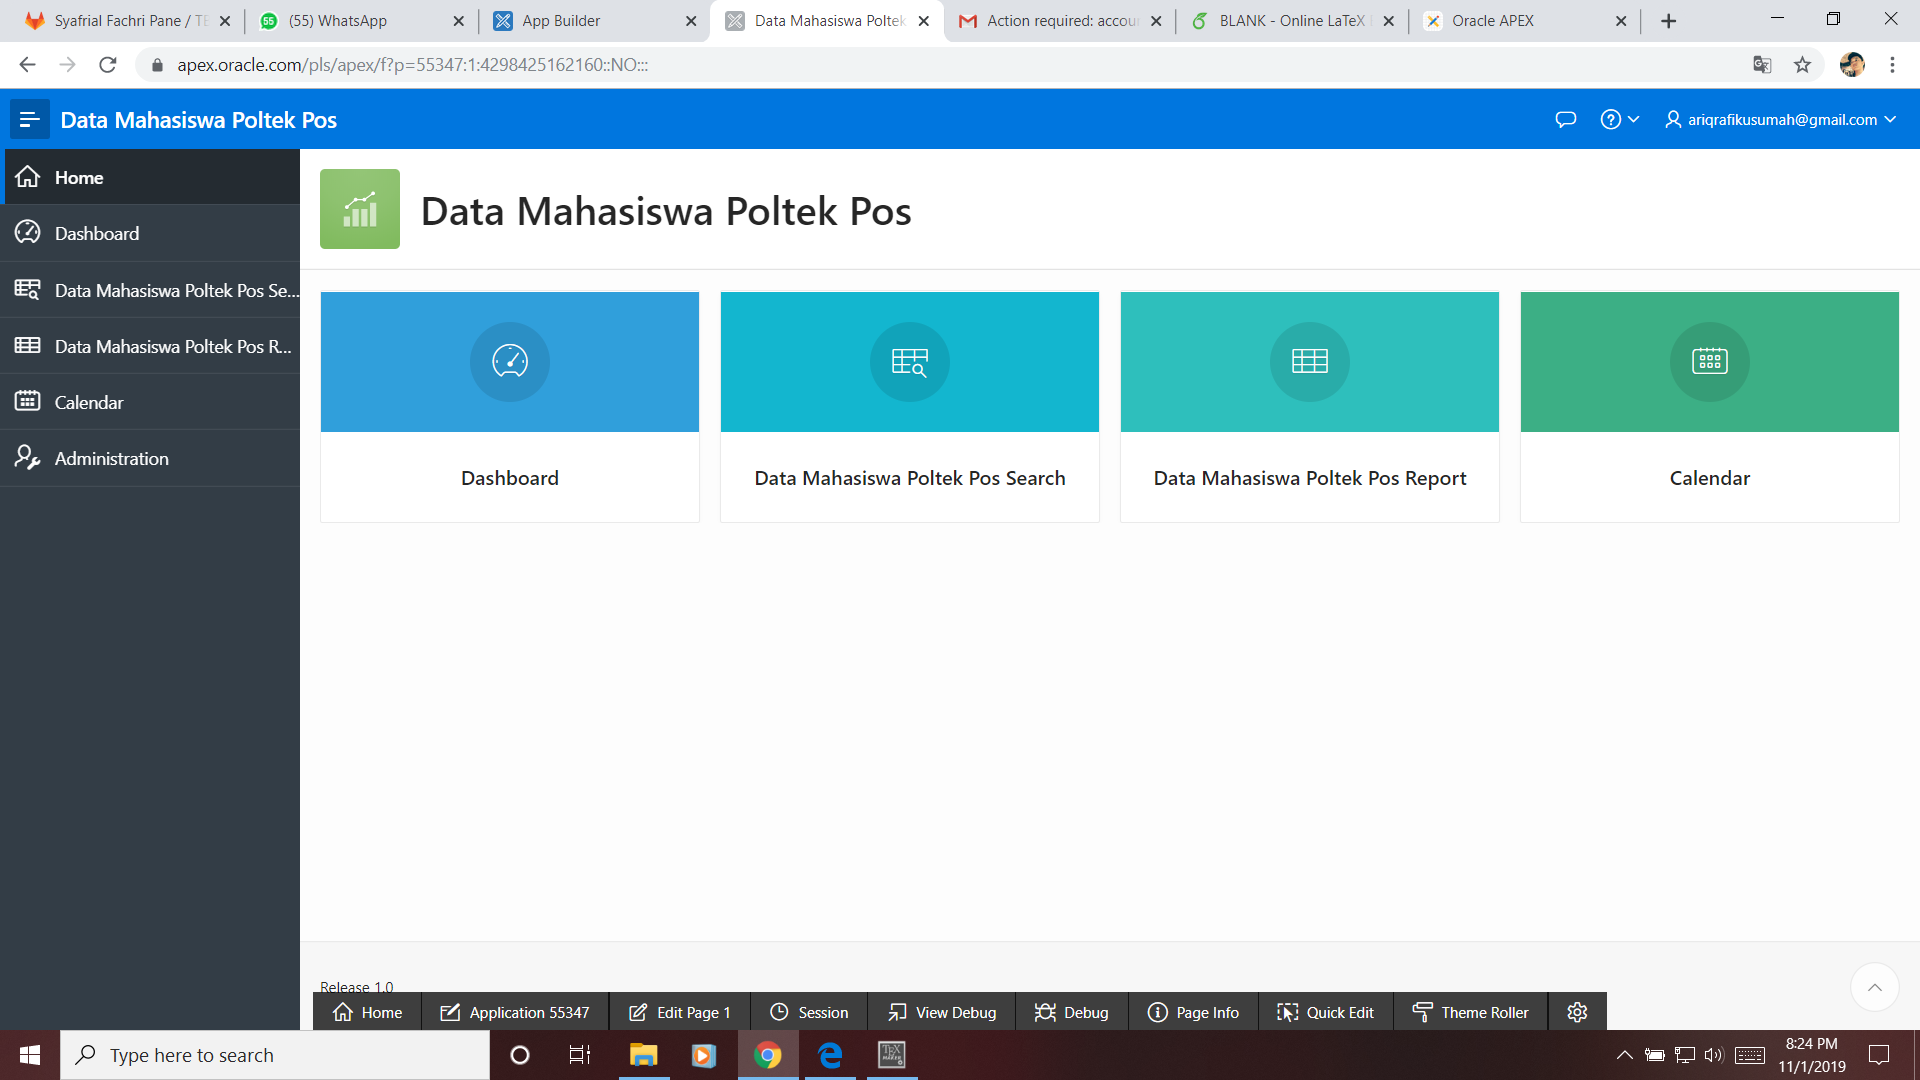
\includegraphics[scale=0.2]{Gambar/Capture16}
	\caption{•}
\end{figure}
\\
\\
\\
\\
\\
\\
\\
\\
\\
\\
\\
\\
\\
\item dan ini data mahasiswanya
\begin{figure}[h]
	\centering
		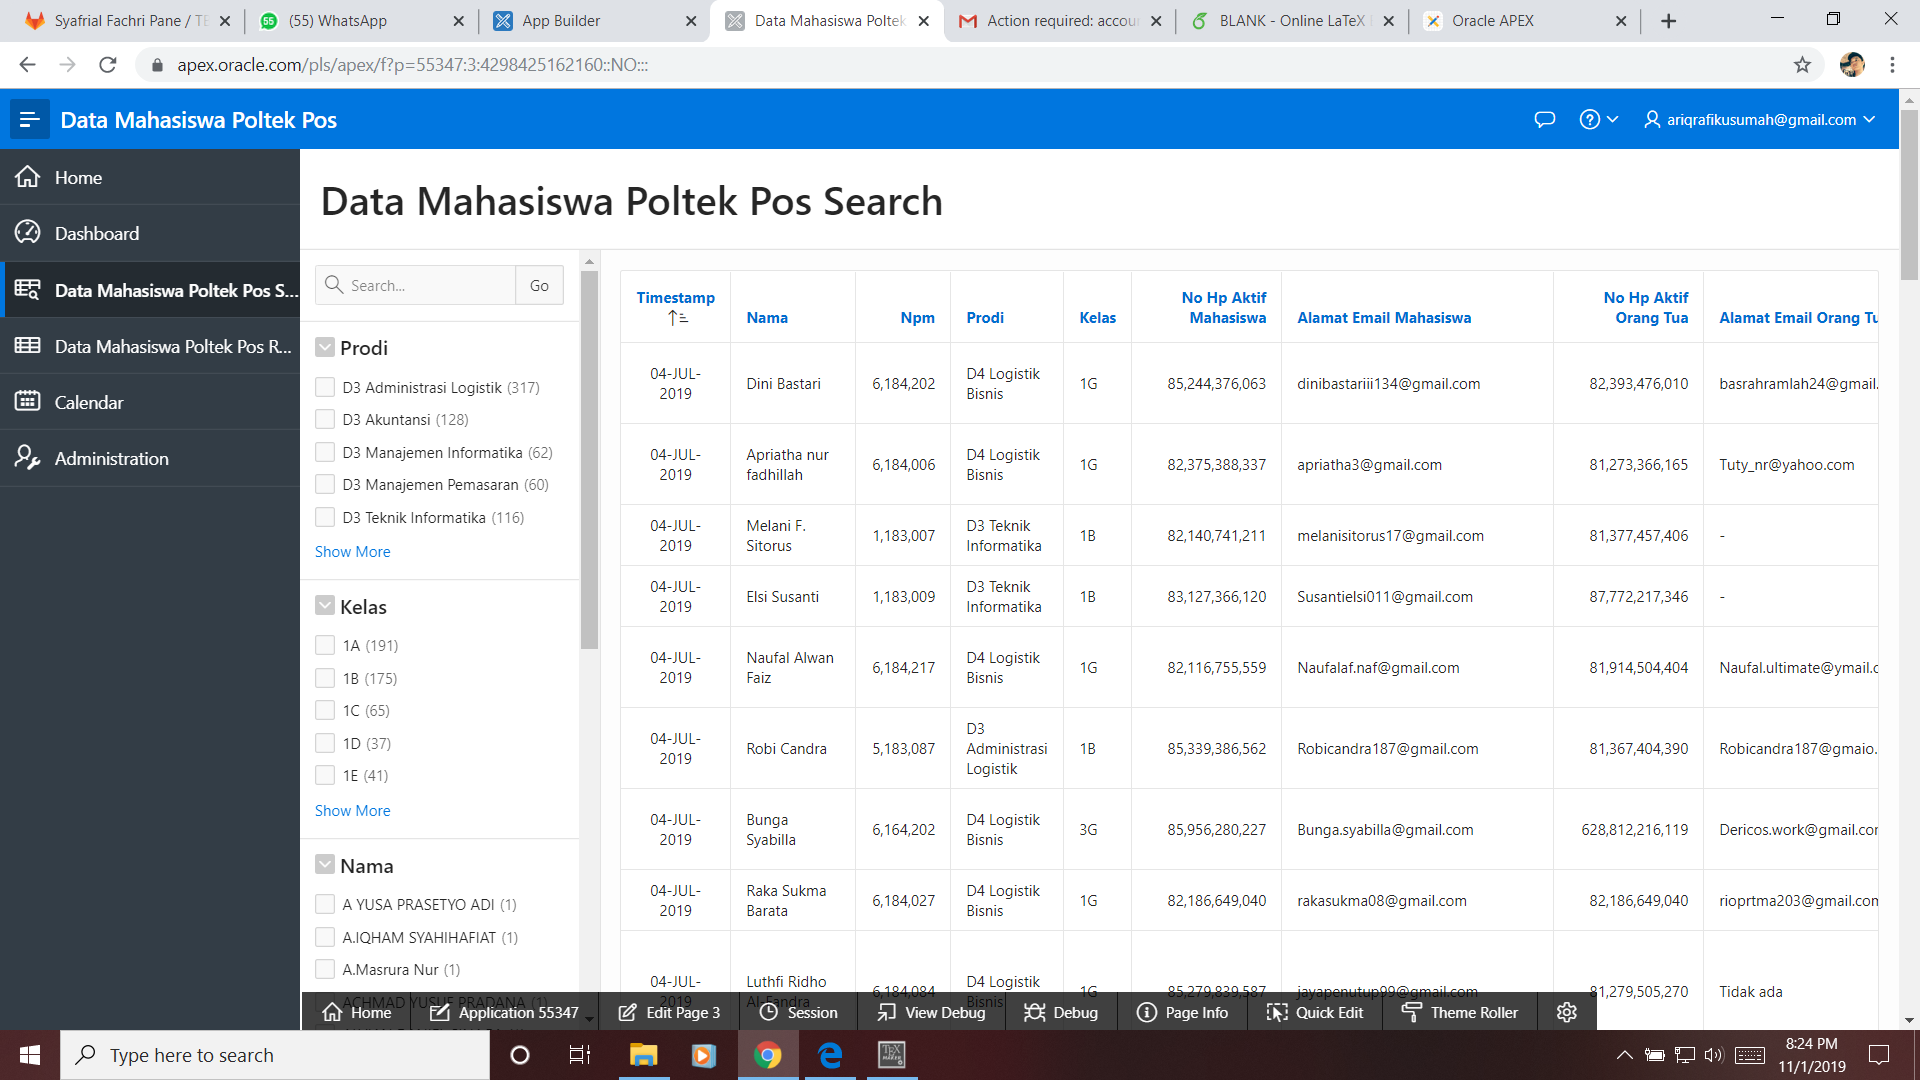
\includegraphics[scale=0.2]{Gambar/Capture17}
	\caption{•}
\end{figure}
\end{enumerate}


\end{document}
